\chapter{Risultati}\label{chap:capitolo4}
\section{Introduzione}
In questo capitolo vengono presentati e discussi i risultati delle analisi numeriche condotte mediante il solutore PFEF sviluppato nei capitoli precedenti. L'obiettivo principale è validare l'efficacia e l'affidabilità del modello nella simulazione della risposta strutturale fortemente non lineare delle reti di funi, valutandone sia le configurazioni di equilibrio sotto carichi statici e peso proprio (\textit{form finding}), sia la capacità di risposta durante prove di carico quasi-statiche. 

La trattazione si articola in due macro-sezioni principali:

\begin{itemize}
    \item \textbf{Reti soggette al peso proprio e carichi statici:} in prima istanza, viene condotta un'ampia indagine parametrica e di sensibilità per comprendere il comportamento del sistema al variare dei principali fattori geometrici, cinematici e meccanici. Nello specifico, si analizza l'effetto delle condizioni di vincolo al bordo applicate alle configurazioni tipiche delle reti di protezione. Viene valutata l'influenza della rigidezza assiale delle funi secondo diverse distribuzioni di sezione. Ampio spazio è dedicato allo studio del fenomeno dello \textit{slack}, mettendo a confronto il comportamento di maglie quadrate e romboidali e illustrando le strategie numeriche implementate per superare la singolarità della matrice di rigidezza. L'analisi statica si completa con la valutazione della risposta della rete sotto l'azione di carichi concentrati, come naturale collegamento con il problema successivo.
    \item \textbf{Simulazione della prova quasi-statica:} Nella seconda parte, il solutore viene applicato alla simulazione della prova quasi-statica, parametro fondamentale per qualificazione energetica del sistema. Vengono dettagliate le caratteristiche geometriche e meccaniche del provino e la storia di carico, concludendo il confronto tra i risultati  numerici e i dati sperimentali per verificare la precisione del modello nel descrivere la risposta globale della rete e la capacità di assorbimento dell'energia di deformazione. 
\end{itemize}

\section{Reti soggette al peso proprio}
In \cref{chap:reti_di_funi}, è stata affrontata la formulazione matematica del metodo agli elementi finiti per le reti di funi, nonché la definizione della matrice di connettività, la quale consente di sviluppare topologie più complesse rispetto a quelle delle semplici funi. 

Successivamente, è emersa la necessità di introdurre specifici strumenti di supporto alla progettazione. Nella presente sezione vengono illustrati gli strumenti sviluppati, concepiti sia per affrontare problematiche progettuali, sia per superare le criticità tipiche del \textit{form-finding} delle reti in bando.

\subsection{Analisi dell'effetto delle condizioni di vincolo al bordo}
Le reti di sicurezza conformi alla normativa EN 1263-1 \cite{EN1263-1} possono essere soggette a molteplici configurazioni di vincolamento esterno. Al fine di poter ripordurre fedelmente tali condizioni all'interno del modello, si rende necessaria una formulazione cinematica versatile che consenta di accoppiare i nodi di bordo della rete con l'ambiente circostante, tenendo conto dei reali gradi di libertà concessi dai sistemi di ancoraggio.

All'interno del solutore sviluppato, le condizioni di vincolo esterne applicabili ai singoli nodi computazionali si basano su due modelli cinematici fondamentali, rappresentati in \cref{fig:confronto_vincoli}.
\begin{itemize}
   \item \textbf{Cerniera fissa} (\cref{fig:confronto_vincoli} (a)): blocca tutti i gradi di libertà traslazionali del nodo ($u_{x_1} = 0, u_{x_2} = 0, u_{x_3} = 0$)
   \item \textbf{Cerniera mobile} (\cref{fig:confronto_vincoli} (b)): l'unico grado di libertà del nodo garantisce la traslazione lungo la direzione dell'asse orizziontale su cui esso giace (es. direzione locale $x_j$), consentendogli lo scorrimento cinematico lungo la guida e bloccando i restanti gradi di libertà ortogonali.
\end{itemize}

\begin{figure}[htbp]
    \centering
    % Contenuto di "143_capitoli/capitolo2/immagini_capitolo_2/confronto_vincoli_3d.tex"
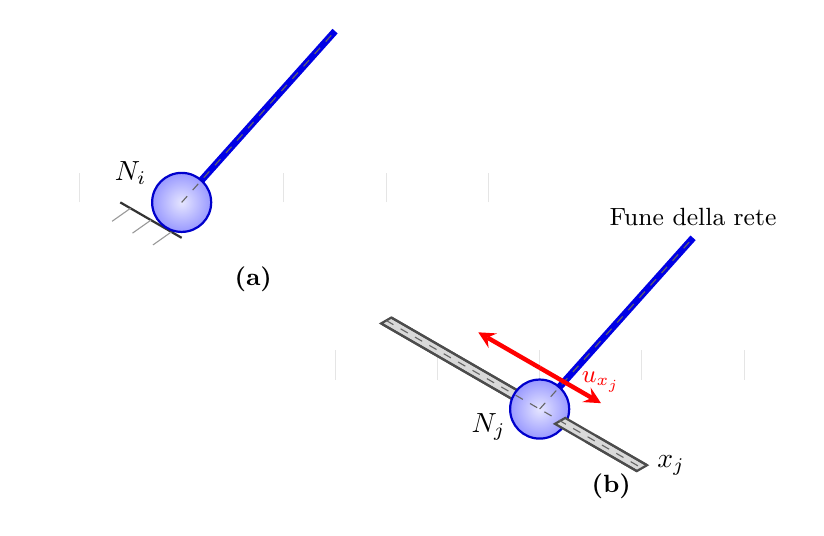
\begin{tikzpicture}[
    scale=1.5,
    x={(0.866cm,-0.5cm)}, y={(0.866cm,0.5cm)}, z={(0cm,1cm)},   % Assonometria isometrica
    guida/.style={draw=black!70, fill=gray!30, thick},
    fune/.style={draw=blue!90!black, line width=2.5pt},
    vettore/.style={->, >=stealth, red, ultra thick},
    titolo/.style={font=\small\bfseries, text=black, align=center}
]

    % =========================================================================
    % 1. SINISTRA: CERNIERA FISSA (Ancorata a terra)
    % =========================================================================
    
    % Piano di fondo locale
    \draw[gray!20, thin, step=0.5] (-1,-0.5,0) grid (1.5,1.5,0);
    
    % Piastra fissa di base a terra (Ancoraggio meccanico strutturale)
    \draw[black!80, thick] (-0.3,-0.3,0) -- (0.3,-0.3,0);
    \foreach \x in {-0.2,0,0.2} {
        \draw[black!40, thin] (\x,-0.3,0) -- (\x-0.08,-0.4,-0.1);
    }

    % Disegno della Fune (prima della sferetta per corretta sovrapposizione)
    \draw[fune] (0,0,0) -- (0.5, 1.0, 1.2);

    % Sferetta del nodo fisso (copre l'inizio della fune)
    \shadedraw[inner color=blue!10, outer color=blue!40, draw=blue!80!black, thick] (0,0,0) circle [radius=0.25cm];

    % Asse della fune (nero tratteggiato, sovrapposto sopra)
    \draw[dashed, black!60, thin] (0,0,0) -- (0.5, 1.0, 1.2);

    % Etichetta del nodo
    \node[black] at (-0.1, -0.4, 0.4) {$N_i$};
    
    % Titolo della subfigura a) bloccato alla quota y=0.5, z=-0.8
    \node[titolo] at (0.2, 0.5, -0.8) {(a)};


    % =========================================================================
    % 2. DESTRA: CERNIERA MOBILE (Su Guida Lineare)
    % =========================================================================
    % Lo shift ora è (3.5, 0, 0) puro: y=0 e z=0 sono identici al precedente.
    % Questo rende le due cerniere perfettamente parallele e complanari.
    \begin{scope}[shift={(3.5,0,0)}]
        
        % Piano di fondo locale
        \draw[gray!20, thin, step=0.5] (-1.5,-0.5,0) grid (1,1.5,0);

        % Guida cilindrica (asse x locale) - parte posteriore
        \fill[guida] (-1.5,-0.05,0) -- (0,-0.05,0) -- (0,0.05,0) -- (-1.5,0.05,0) -- cycle;
        \draw[black!70, thick] (-1.5,-0.05,0) -- (0,-0.05,0);
        \draw[black!70, thick] (-1.5,0.05,0) -- (0,0.05,0);

        % Disegno della Fune
        \draw[fune] (0,0,0) -- (0.5, 1.0, 1.2) node[above, black] {\small Fune della rete};

        % Sferetta del nodo mobile (copre l'inizio della fune e la parte posteriore della guida)
        \shadedraw[inner color=blue!10, outer color=blue!40, draw=blue!80!black, thick] (0,0,0) circle [radius=0.25cm];

        % Parte anteriore della guida
        \fill[guida] (0.2,-0.05,0) -- (1.0,-0.05,0) -- (1.0,0.05,0) -- (0.2,0.05,0) -- cycle;
        \draw[black!70, thick] (0.5,-0.05,0) -- (1.0,-0.05,0);
        \draw[black!70, thick] (0.5,0.05,0) -- (1.0,0.05,0) node[right, black] {$x_j$};
     
        % Asse geometrico della guida
        \draw[dashed, black!60, thin] (-1.5,0,0) -- (1.0,0,0);

        % Asse della fune (nero tratteggiato)
        \draw[dashed, black!60, thin] (0,0,0) -- (0.5, 1.0, 1.2);

        % Frecce dei Gradi di Libertà (Traslazione u_xj)
        \draw[vettore] (0,0,0.35) -- (0.6,0,0.35) node[above] {\small $u_{x_j}$};
        \draw[vettore] (0,0,0.35) -- (-0.6,0,0.35);

        % Etichetta del nodo
        \node[black] at (-0.1, -0.4, 0) {$N_j$};
        
        % Titolo della subfigura b) bloccato alla stessa identica coordinata relativa
        \node[titolo] at (0.2, 0.5, -0.8) {(b)};
        
    \end{scope}

\end{tikzpicture}
    \caption{Vincoli cinematici: (a) -  Cerniera fissa (spostamenti impediti), (b) - Cerniera scorrevole (scorrimento lungo $x_j$)}
    \label{fig:confronto_vincoli}
\end{figure}

Oltre alla natura cinematica del vincolo applicato, il solutore offre una struttura per la selezione della geometria dei vincoli. Nello specifico, l'utente può scegliere tra quattro diverse distribuzioni spaziali dei nodi vincolati:
\begin{itemize}
   \item \textbf{Vincolo perimetrale completo:} la condizione di cerniera (fissa o scorrevole) viene estesa a tutti i nodi appartenenti ai quattro lati esterni della maglia (vedi \cref{fig:rete_vincolata_4lati});
   \item \textbf{Vincolo su 2 lati paralleli:} (direzione $x$ o $y$): il vincolamento viene attivato esclusivamente per i nodi disposti lungo i bordi paralleli ad un singolo asse del dominio, lasciando liberi i restanti due margini (vedi \cref{fig:rete_vincolata_x,fig:rete_vincolata_y}). Questa specifica configurazione riveste un importanza notevole nel campo delle \textit{Safety nets}, poichè riproduce le condizioni di vincolo tipiche delle reti di \textit{Sistema T} e \textit{Sistema U}. 
   
   Dal punto di vista numerico, mentre l'impiego di cerniere fisse garantisce la stabilità della mesh, l'utilizzo di cerniere scorrevoli, frequente in questa tipologia di applicazioni, rende la soluzione del problema originariamente indeterminata a causa della comparsa di moti rigidi globali del sistema in direzione dell'asse vincolato. Per ovviare a tale problematica e restituire l'unicità della soluzione, nel solutore è introdotta una regolarizzazione del legame costitutivo che simula una seppur irrisoria trazione degli elementi fune o, più verosimilmente, l'aliquota di resistenza attritiva e di contatto opposta dal vincolo sulle funi adiacenti. 
   Tuttavia, sebbene la regolarizzazione eviti la singolarità della matrice garantendo la convergenza del solutore, lo scorrimento incontrollato dei nodi di bordo rischia di condurre ad una soluzione priva di senso fisico, caratterizzata da un eccessivo trasversale. Per impedire tale eventualità e preservare la coerenza con la configurazione di progetto, i quattro nodi d'angolo vengono vincolati mediante cerniere fisse.
   \item \textbf{vincolo sui 4 vertici d'angolo:} la condizione di vincolo si applica strettamente ai 4 nodi d'estremità che identificano gli angoli della rete (\cref{fig:rete_vincolata_corners}). Questa specifica configurazione riveste una notevole importanza ingegneristica, poichè riproduce la condizione di vincolo delle reti di \textit{Sistema S} soggette al test di impatto dinamico previsto dalla norma EN 1263-1 \cite{EN1263-1}.
\end{itemize}

La risposta strutturale del sistema è investigata assumendo come riferimento una rete a maglia quadrata (Q) con le caratteristiche geometriche e meccaniche riportate in \cref{tab:caratteristiche_vincoli_rete}.
\begin{figure}[H]
    \centering
    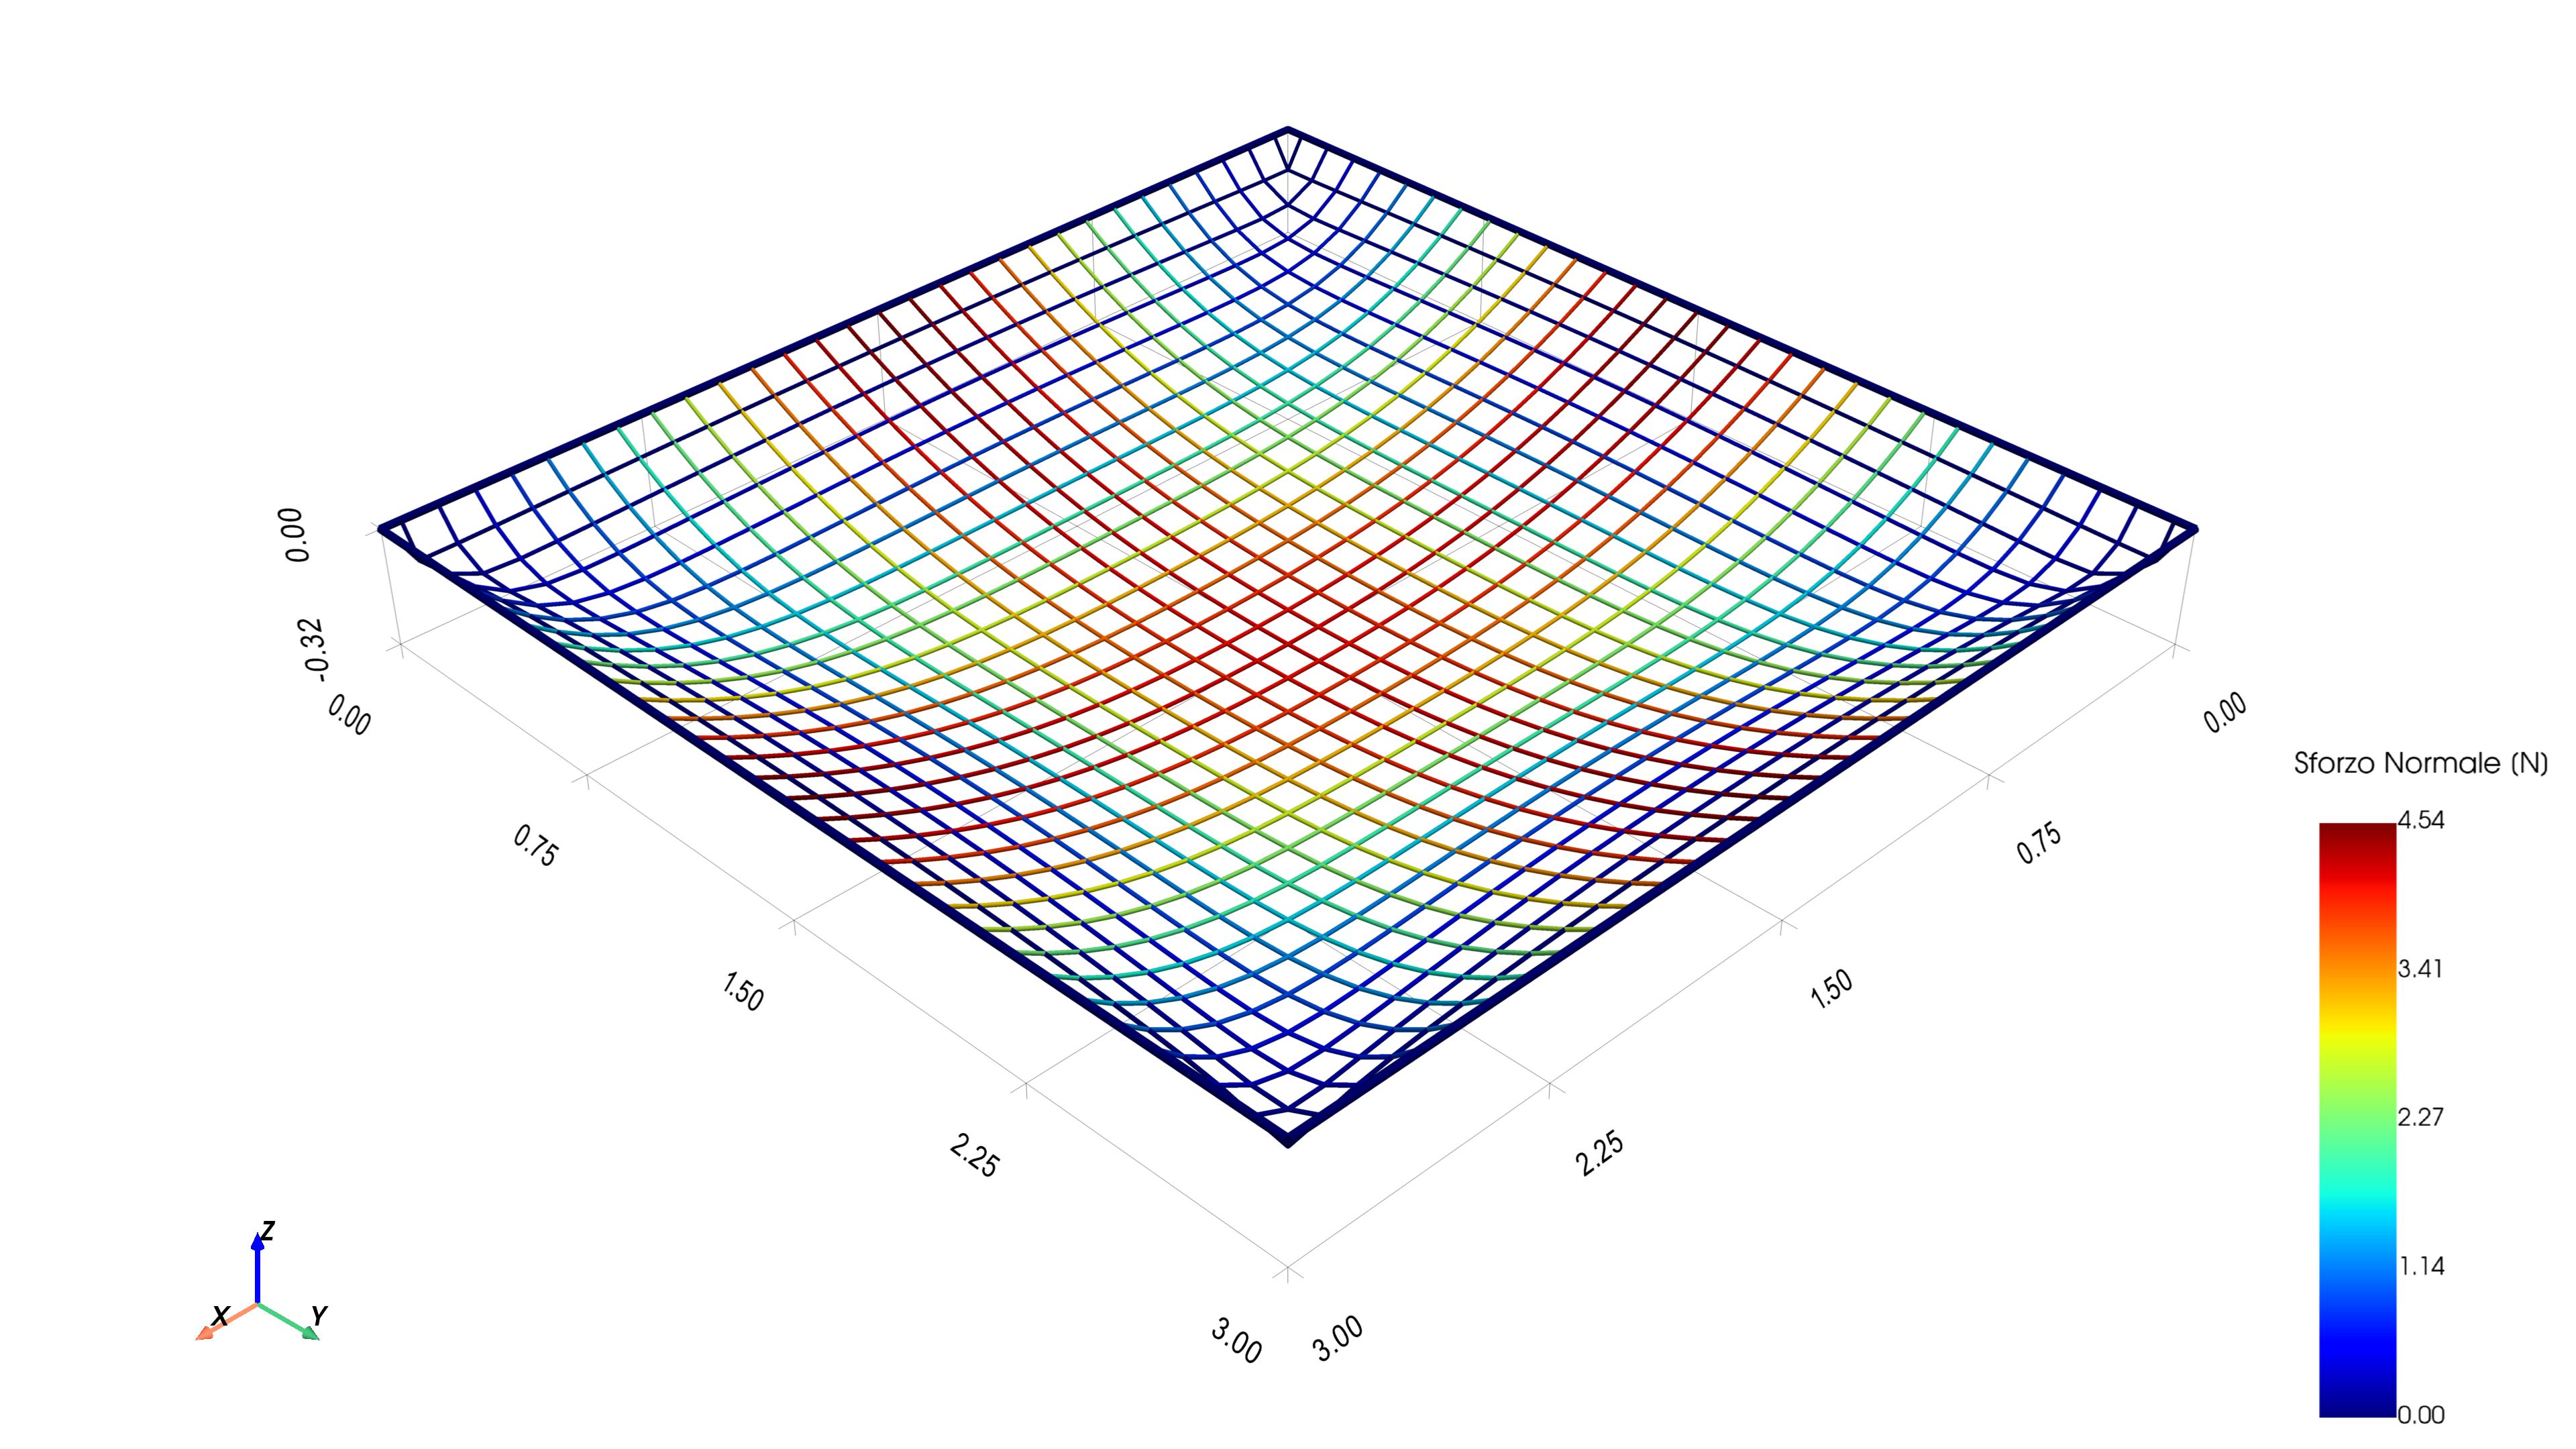
\includegraphics[width=\textwidth]{143_capitoli/capitolo4/immagini_capitolo_4/immagini_vincoli/rete_vincolata_4lati.png}
    \caption{Rete vincolata su 4 lati con cerniere mobili}
    \label{fig:rete_vincolata_4lati}
\end{figure}

\begin{figure}[H]
    \centering
    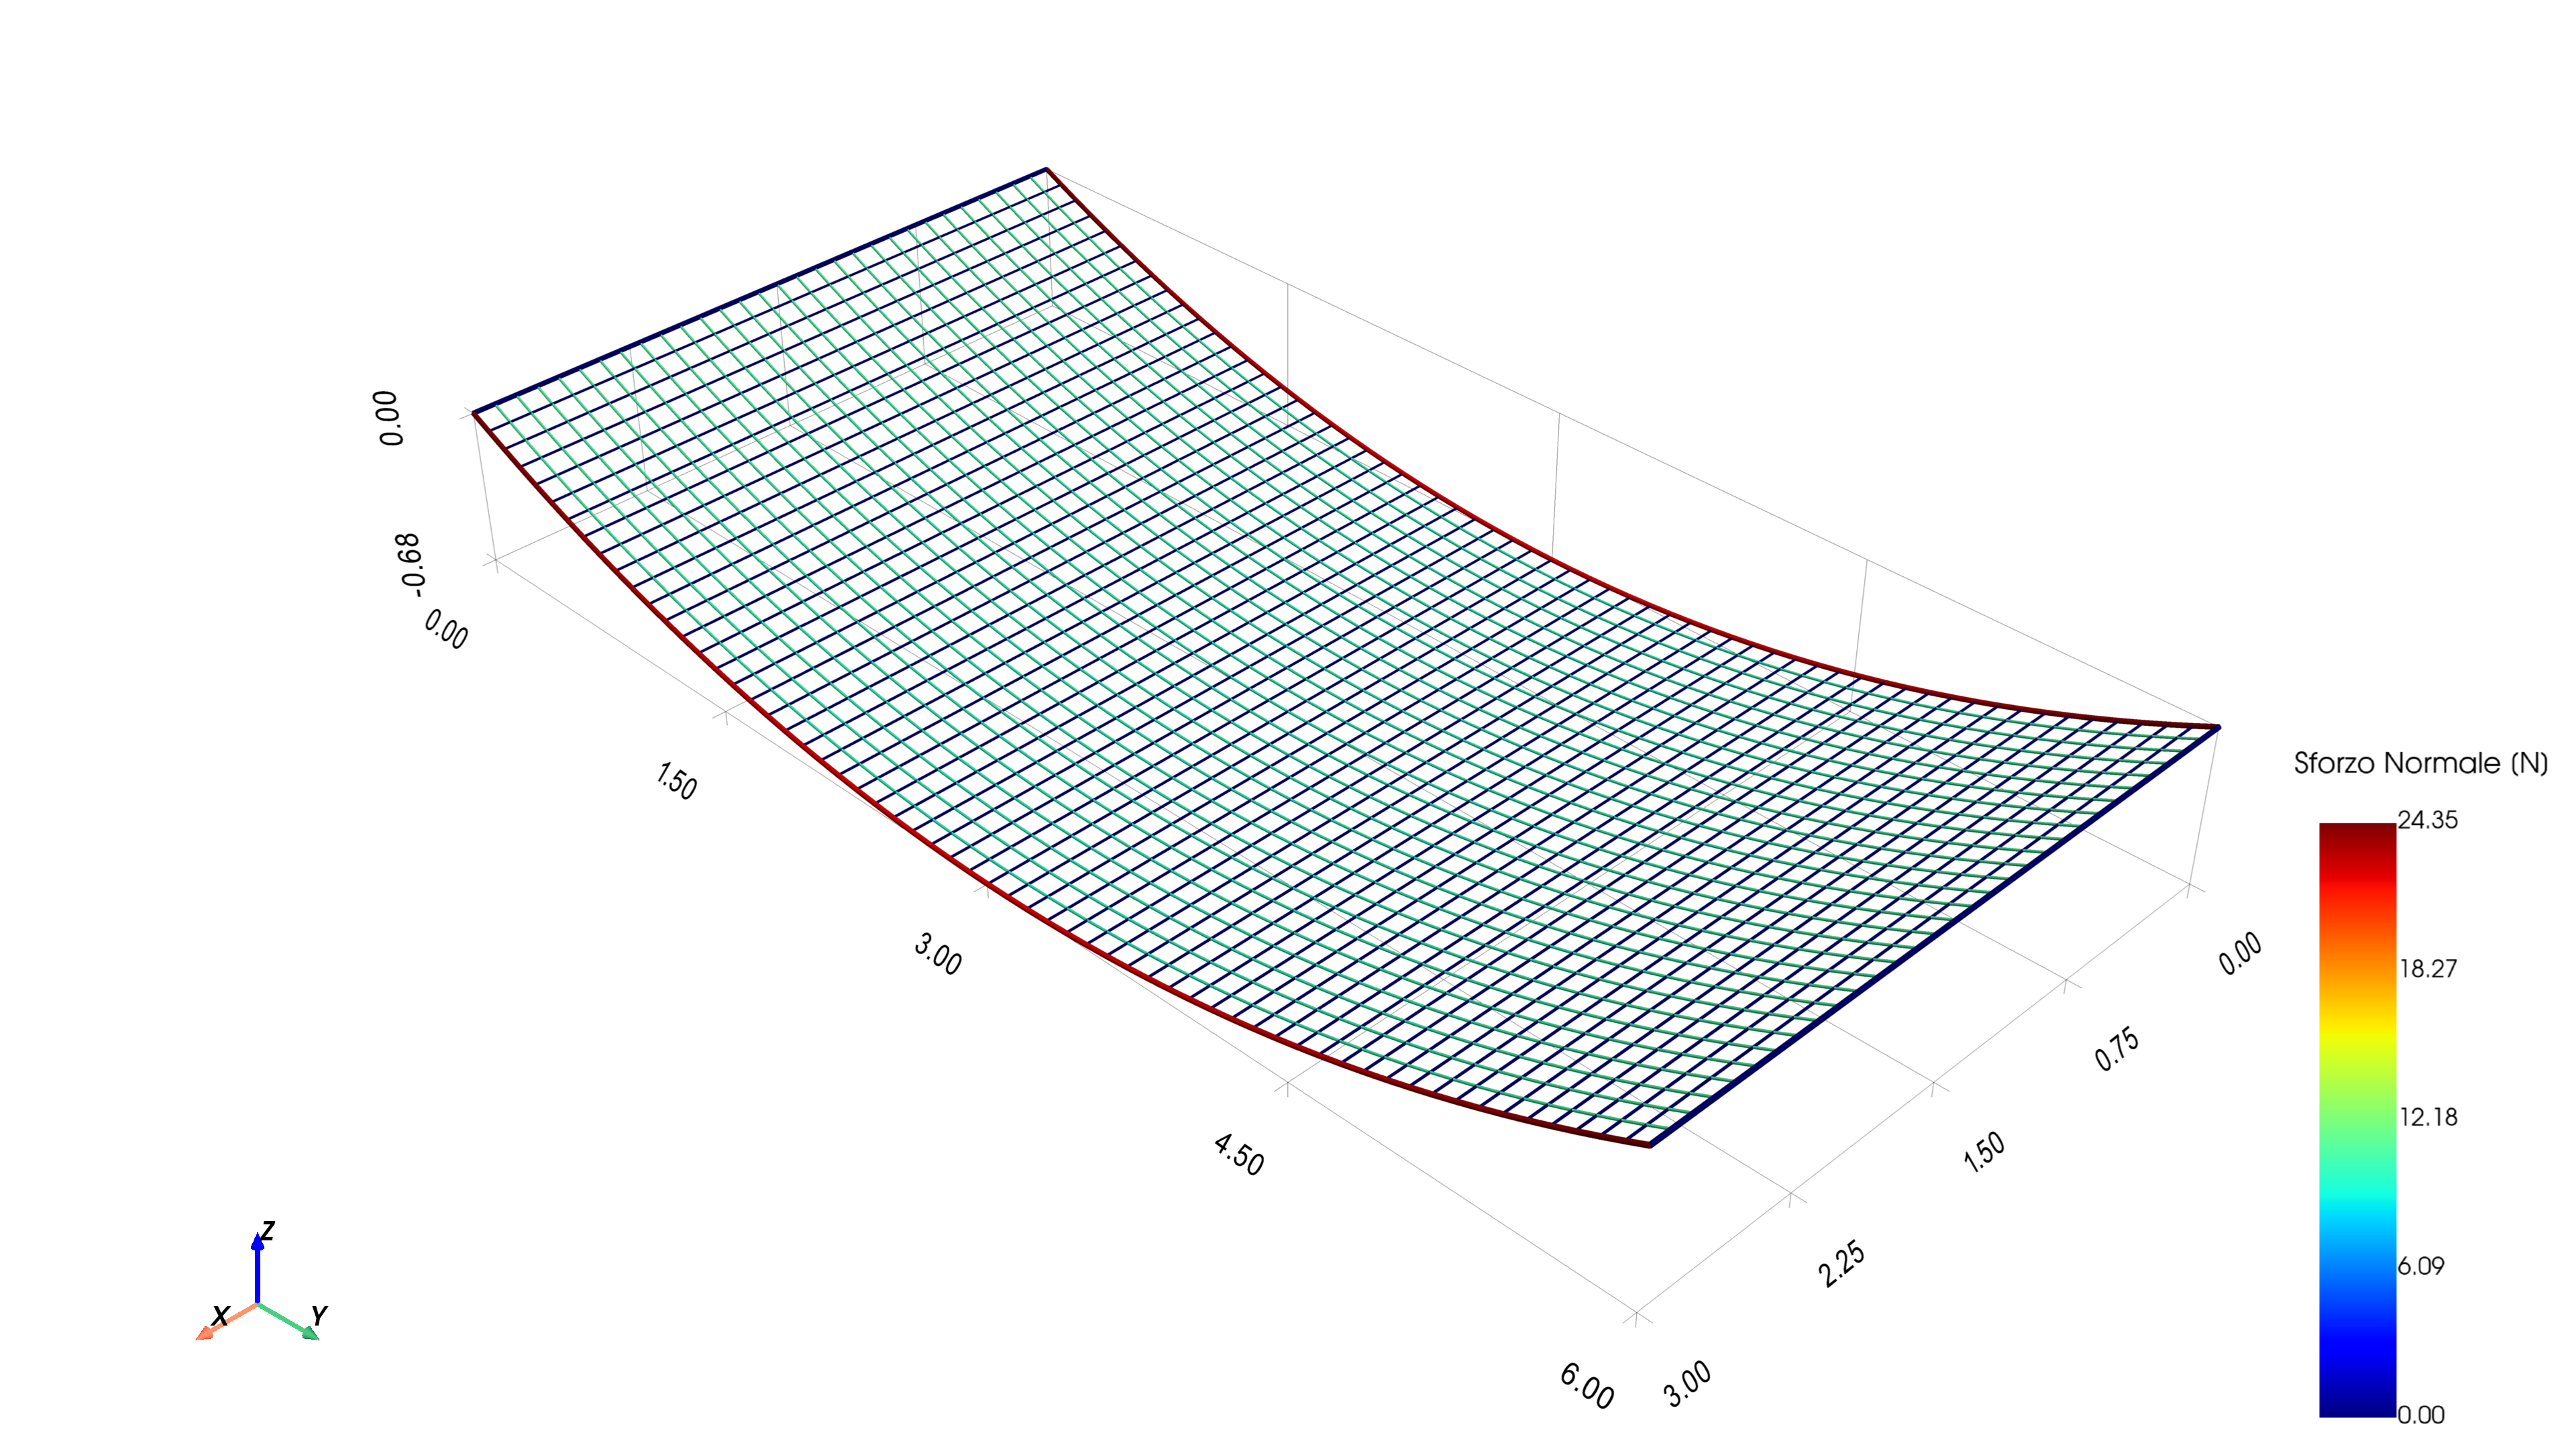
\includegraphics[width=\textwidth]{143_capitoli/capitolo4/immagini_capitolo_4/immagini_vincoli/rete_vincolata_x.png}
    \caption{Rete vincolata lungo i lati paralleli alla direzione 'x'}
    \label{fig:rete_vincolata_x}
\end{figure}

\begin{figure}[H]
    \centering
    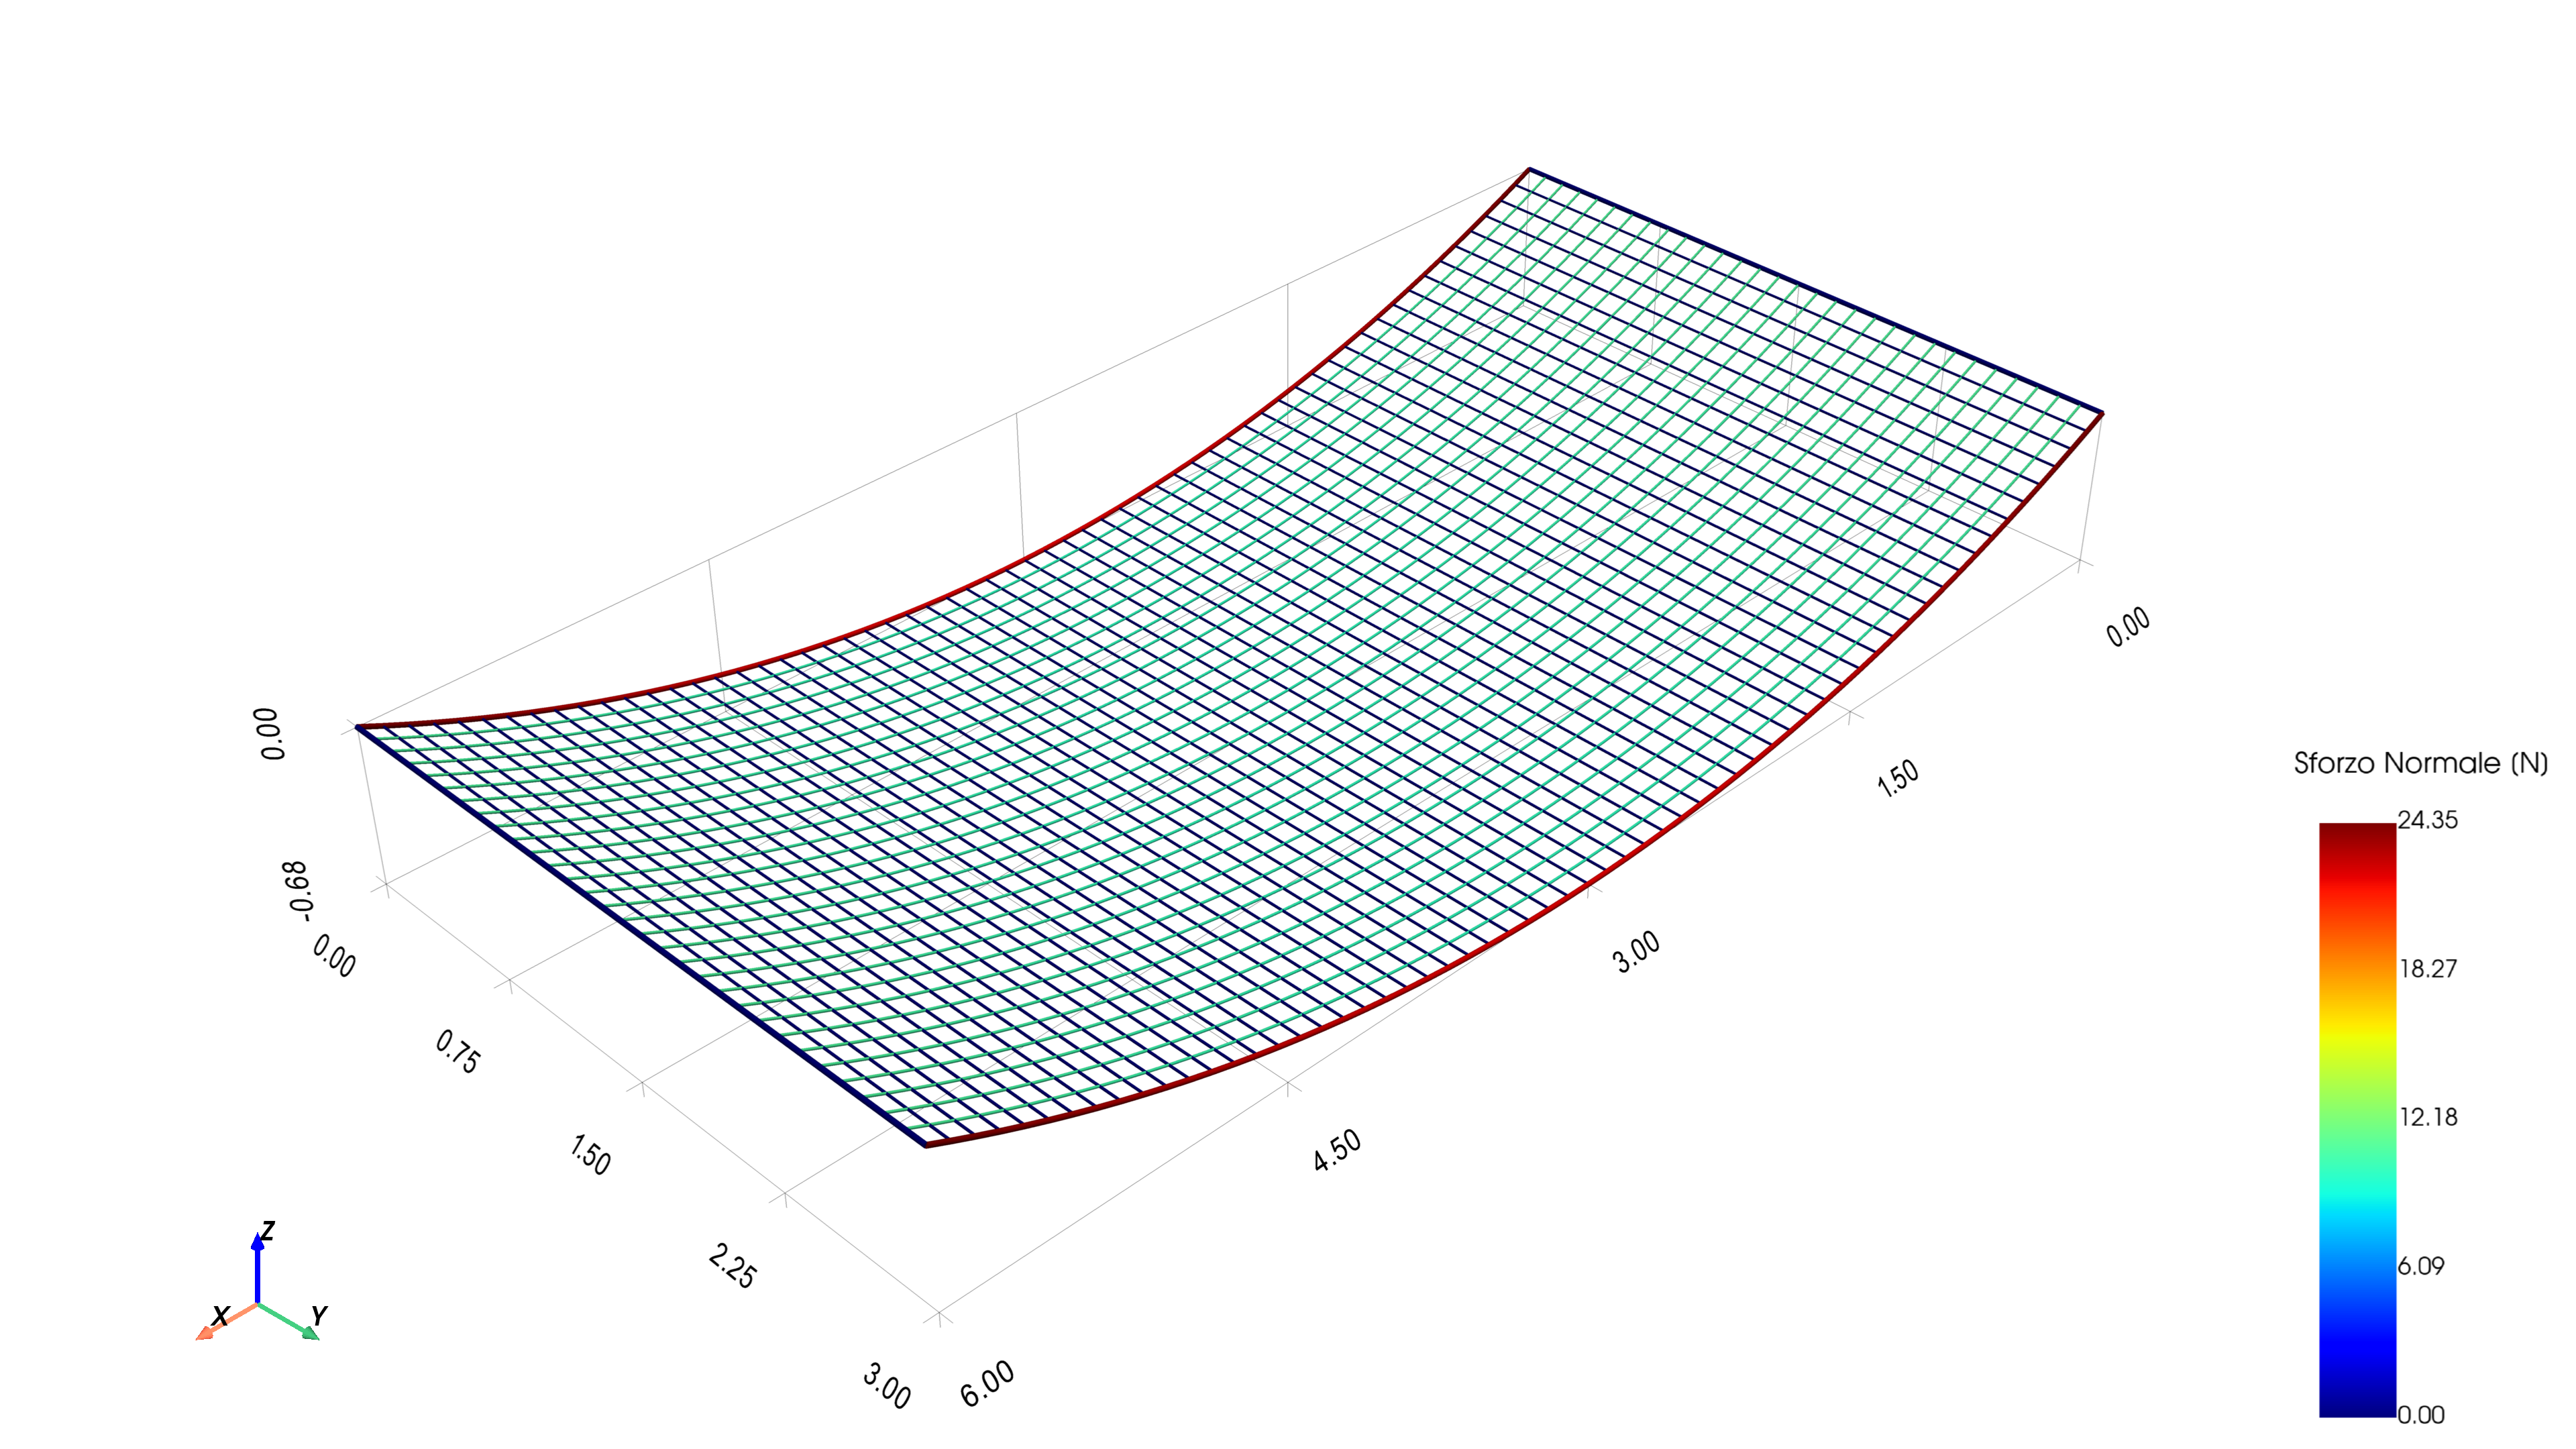
\includegraphics[width=\textwidth]{143_capitoli/capitolo4/immagini_capitolo_4/immagini_vincoli/rete_vincolata_y.png}
    \caption{Rete vincolata lungo i lati paralleli alla direzione 'y'}
    \label{fig:rete_vincolata_y}
\end{figure}

\begin{figure}[H]
    \centering
    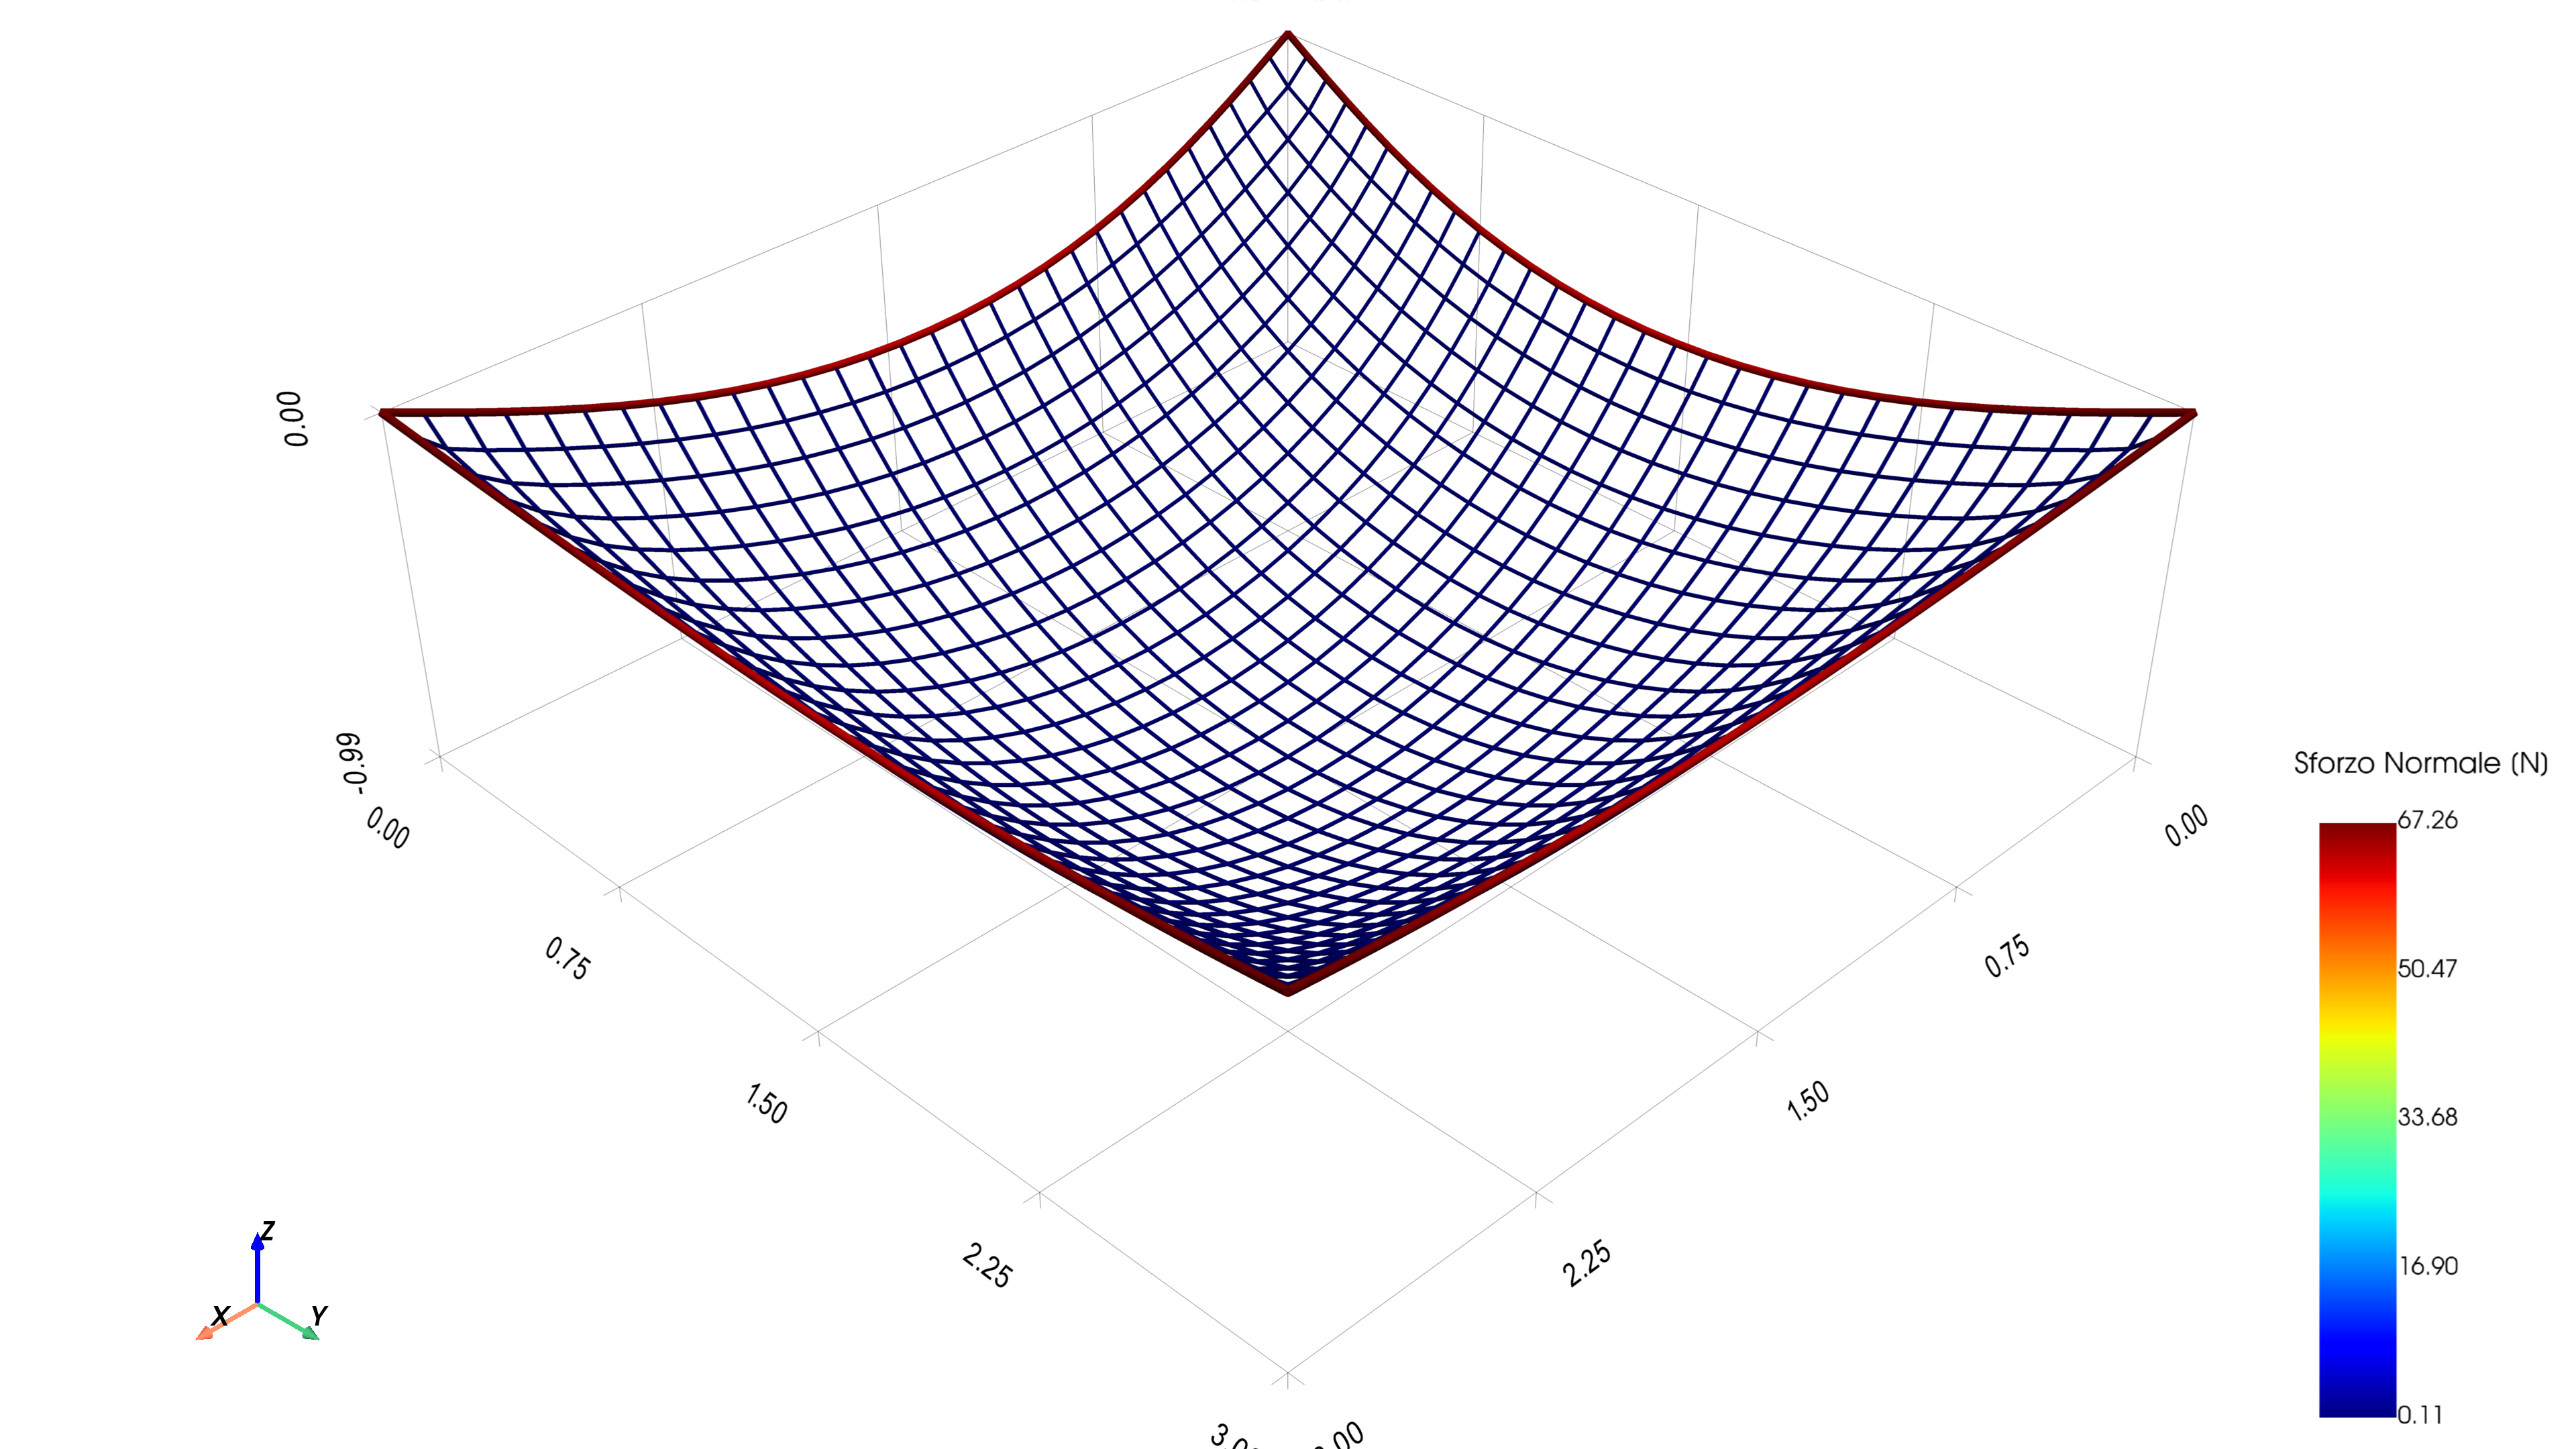
\includegraphics[width=\textwidth]{143_capitoli/capitolo4/immagini_capitolo_4/immagini_vincoli/rete_vincolata_corners.png}
    \caption{Rete vincolata ai nodi d'angolo}
    \label{fig:rete_vincolata_corners}
\end{figure}

\begin{table}[htbp]
    \centering
    \caption{Proprietà geometriche e meccaniche delle reti in \cref{fig:rete_vincolata_4lati,fig:rete_vincolata_x,fig:rete_vincolata_y,fig:rete_vincolata_corners}}
    \vspace{5pt}
    \label{tab:caratteristiche_vincoli_rete}
    \begin{tabularx}{\textwidth}{l c X}
        \hline
        \textbf{Parametro} & \textbf{Simbolo} & \textbf{Valore nominale} \\ \hline
        Dimensione totale della rete & $L_x \times L_y$ & Vedi l'immagine $[\text{m}]$ \\
        Dimensione della singola maglia & $l_{m_x} \times l_{m_y}$ & $10 \times 10$ $[\text{cm}]$ \\
        Diametro nominale delle funi di maglia & $\phi_1$ & $5.0$ $[\text{mm}]$ \\
        Diametro nominale delle funi di bordo & $\phi_2$ & $10.0$ $[\text{mm}]$ \\
        Area sezione trasversale fune di maglia & $A_1$ & 19.63 $[\text{mm}^2]$ \\
        Area sezione trasversale fune di bordo & $A_2$ & 78.54 $[\text{mm}^2]$ \\
        Modulo di elasticità longitudinale fune & $E$ & 2.1e9 $[\text{Pa}]$ \\
        Regolarizzazione del legame costitutivo & $\beta$ & 1e9 $[-]$\\       
        Rapporto di laschezza in entrambe le direzioni & $\xi$& 3.33 $[\text{\%}]$\\ \hline
    \end{tabularx}
\end{table}

\subsection{Influenza della rigidezza assiale delle funi}
La distribuzione delle forze all'interno di un sistema iperstatico è influenzata dalla ripartizione della rigidezza elastica tra gli elementi strutturali partecipanti. 

Nel caso specifico di strutture a comportamento fortemente non lineare per geometria, in cui l'ipotesi di piccoli spostamenti decade, la risoluzione numerica richiede l'impiego della matrice di rigidezza tangente, definita secondo l'\cref{eq:rigidezza_meccanica_geometrica}. Tale operatore risulta funzione diretta della rigidezza assiale degli elementi e della loro distribuzione spaziale. Di conseguenza, la corretta applicazione delle proprietà sezionali delle funi governa sia l'evoluzione delle stato tensionale sia la convergenza del processo iterativo volto alla soluzione del problema non lineare. 

All'interno del solutore, la rigidezza assiale degli elementi è modellata assumendo il modulo di elasticità $E$ costante in funzione del materiale impiegato e variando l'area trasversale efficace $A$ mediante la definizione di un raggio fittizio dei cavi. E'necessario evidenziare come il raggio imposta alla sezione circolare degli elementi sia un parametro puramente fittizio: le funi reali, infatti, non sono costituite da solidi omogenei a sezione piena, bensì da trefoli orditi secondo specifiche configurazioni geometriche. La presenza di vuoti interstiziali e lo scorrimento relativo tra i fili fanno sì che l'area resistente effettiva $A$ e il modulo elastico equivalente $E$ differiscano significativamente dai corrispondenti valori geometrici di un cilindro compatto di pari diametro. 

Tuttavia, l'assunzione di un comportamento elastico lineare per il materiale (ipotesi pienamente verificata per i problemi di validazione analizzati nel presente paragrafo, in cui le reti sono soggette al solo peso proprio o a carichi concentrati di intensità contenuta) consente di ottenere risultati fisicamente realistici e proporzionali alla rigidezza relativa dei componenti. Sotto l'ipotesi che la variabilità della rigidezza reale sia correlata linearmente alla sezione efficace, il solutore descrive con sufficiente accuratezza il flusso delle forze interne in funzione dei rapporti di rigidezza imposti. 

Il solutore consente di modellare diverse distribuzioni di area trasversale:
\begin{itemize}
   \item \textbf{Configurazione omogenea:} tutti gli elementi fune del dominio presentano la stessa area trasversale;
   \item \textbf{Configurazione differenziata a due vie:} distinzione di proèprietà tra le funi costituenti la maglia interna e le funi di bordo (\textit{border rope});
   \item \textbf{Configurazione differenziata a tre vie:} si ha una caratterizzazione indipendendente per le funi di maglia, le funi di bordo e le funi poste sulle diagonali principali, ove presenti. 
\end{itemize}
Sulla base dello scenario voluto l'algoritmo genera un vettore che associa a ciascun elemento strutturale l'area della sezione trasversale, sfruttando l'ordinamento degli elementi visto in \cref{chap:connettività}. Sviluppi futuri del codice potranno includere mappature ancor più flessibili a supporto della pregettazione. 

I risultati relativi ad una rete a maglia quadrata con funi di controvento vincolata ai 4 nodi d'angolo, le cui caratteristiche geometriche e meccaniche sono riassunte in \cref{tab:caratteristiche_area_rete}, sono riportati nelle \cref{fig:rete_aree_uguali,fig:rete_aree_diffenti1,fig:rete_aree_differenti2}.

\begin{figure}[H]
    \centering
    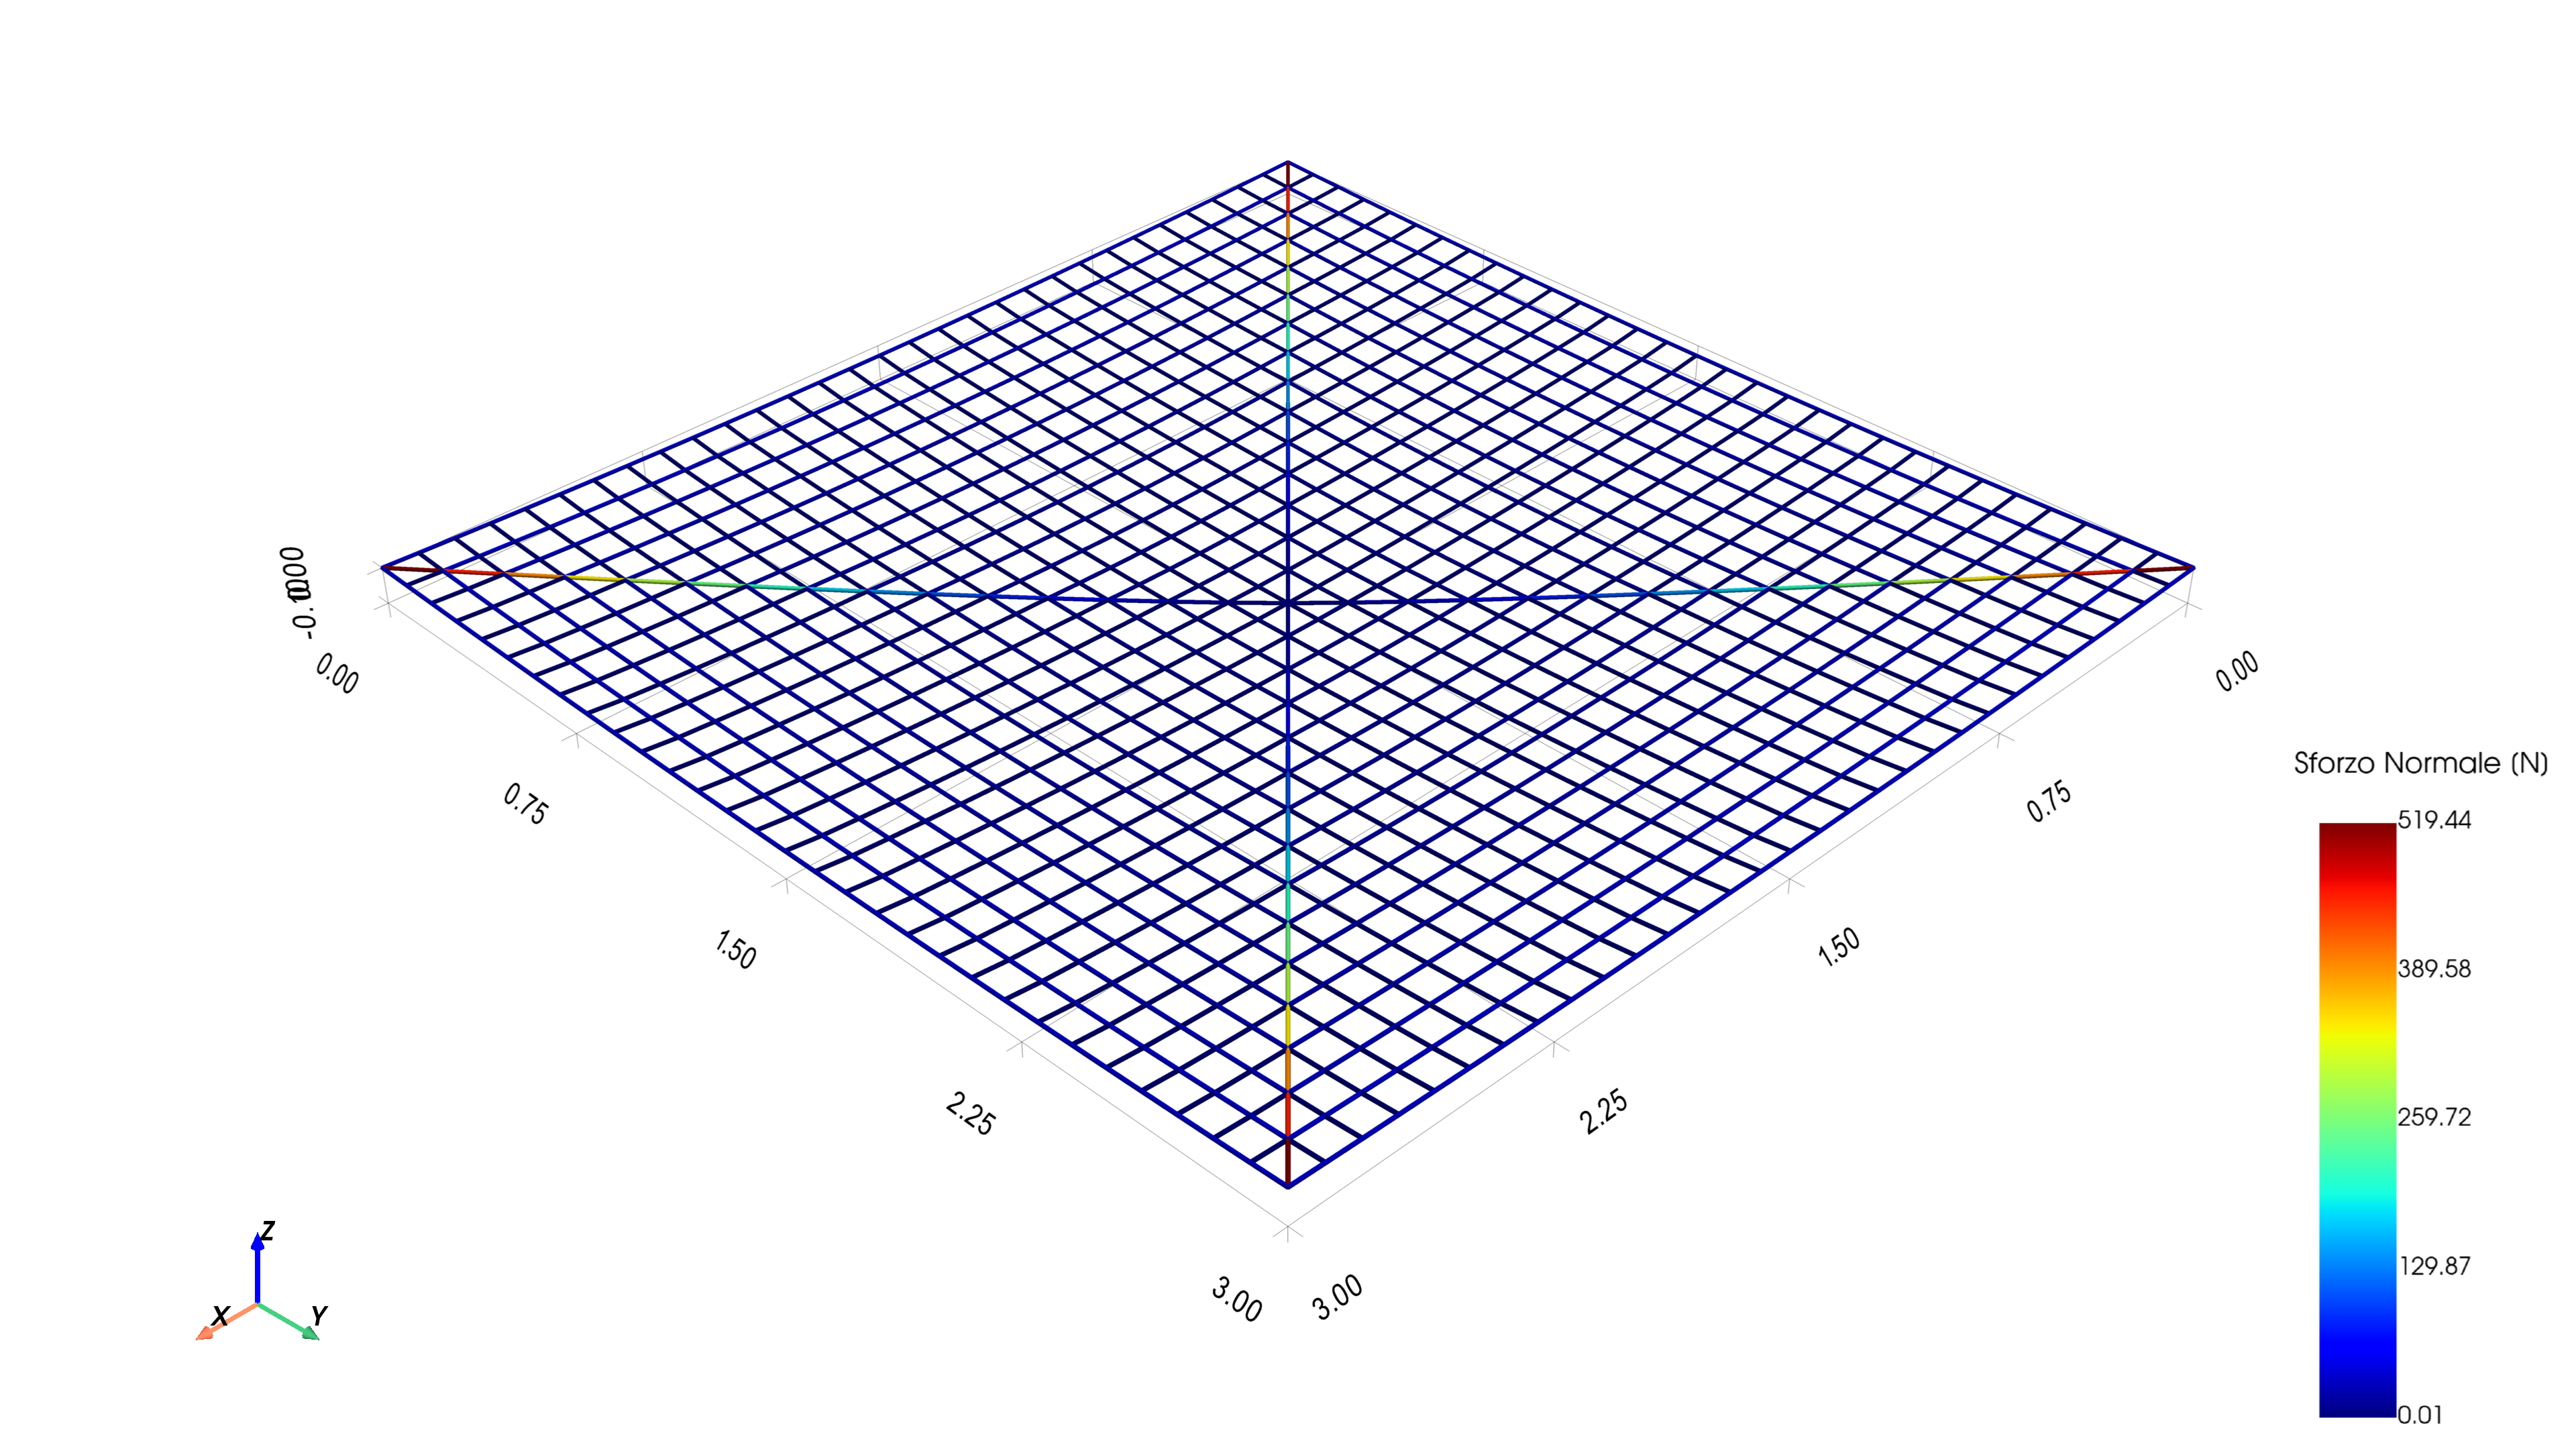
\includegraphics[width=\textwidth]{143_capitoli/capitolo4/immagini_capitolo_4/immagini_area/rete_aree_uguali.png}
    \caption{Rete con configurazione omogenea}
    \label{fig:rete_aree_uguali}
\end{figure}

\begin{figure}[H]
    \centering
    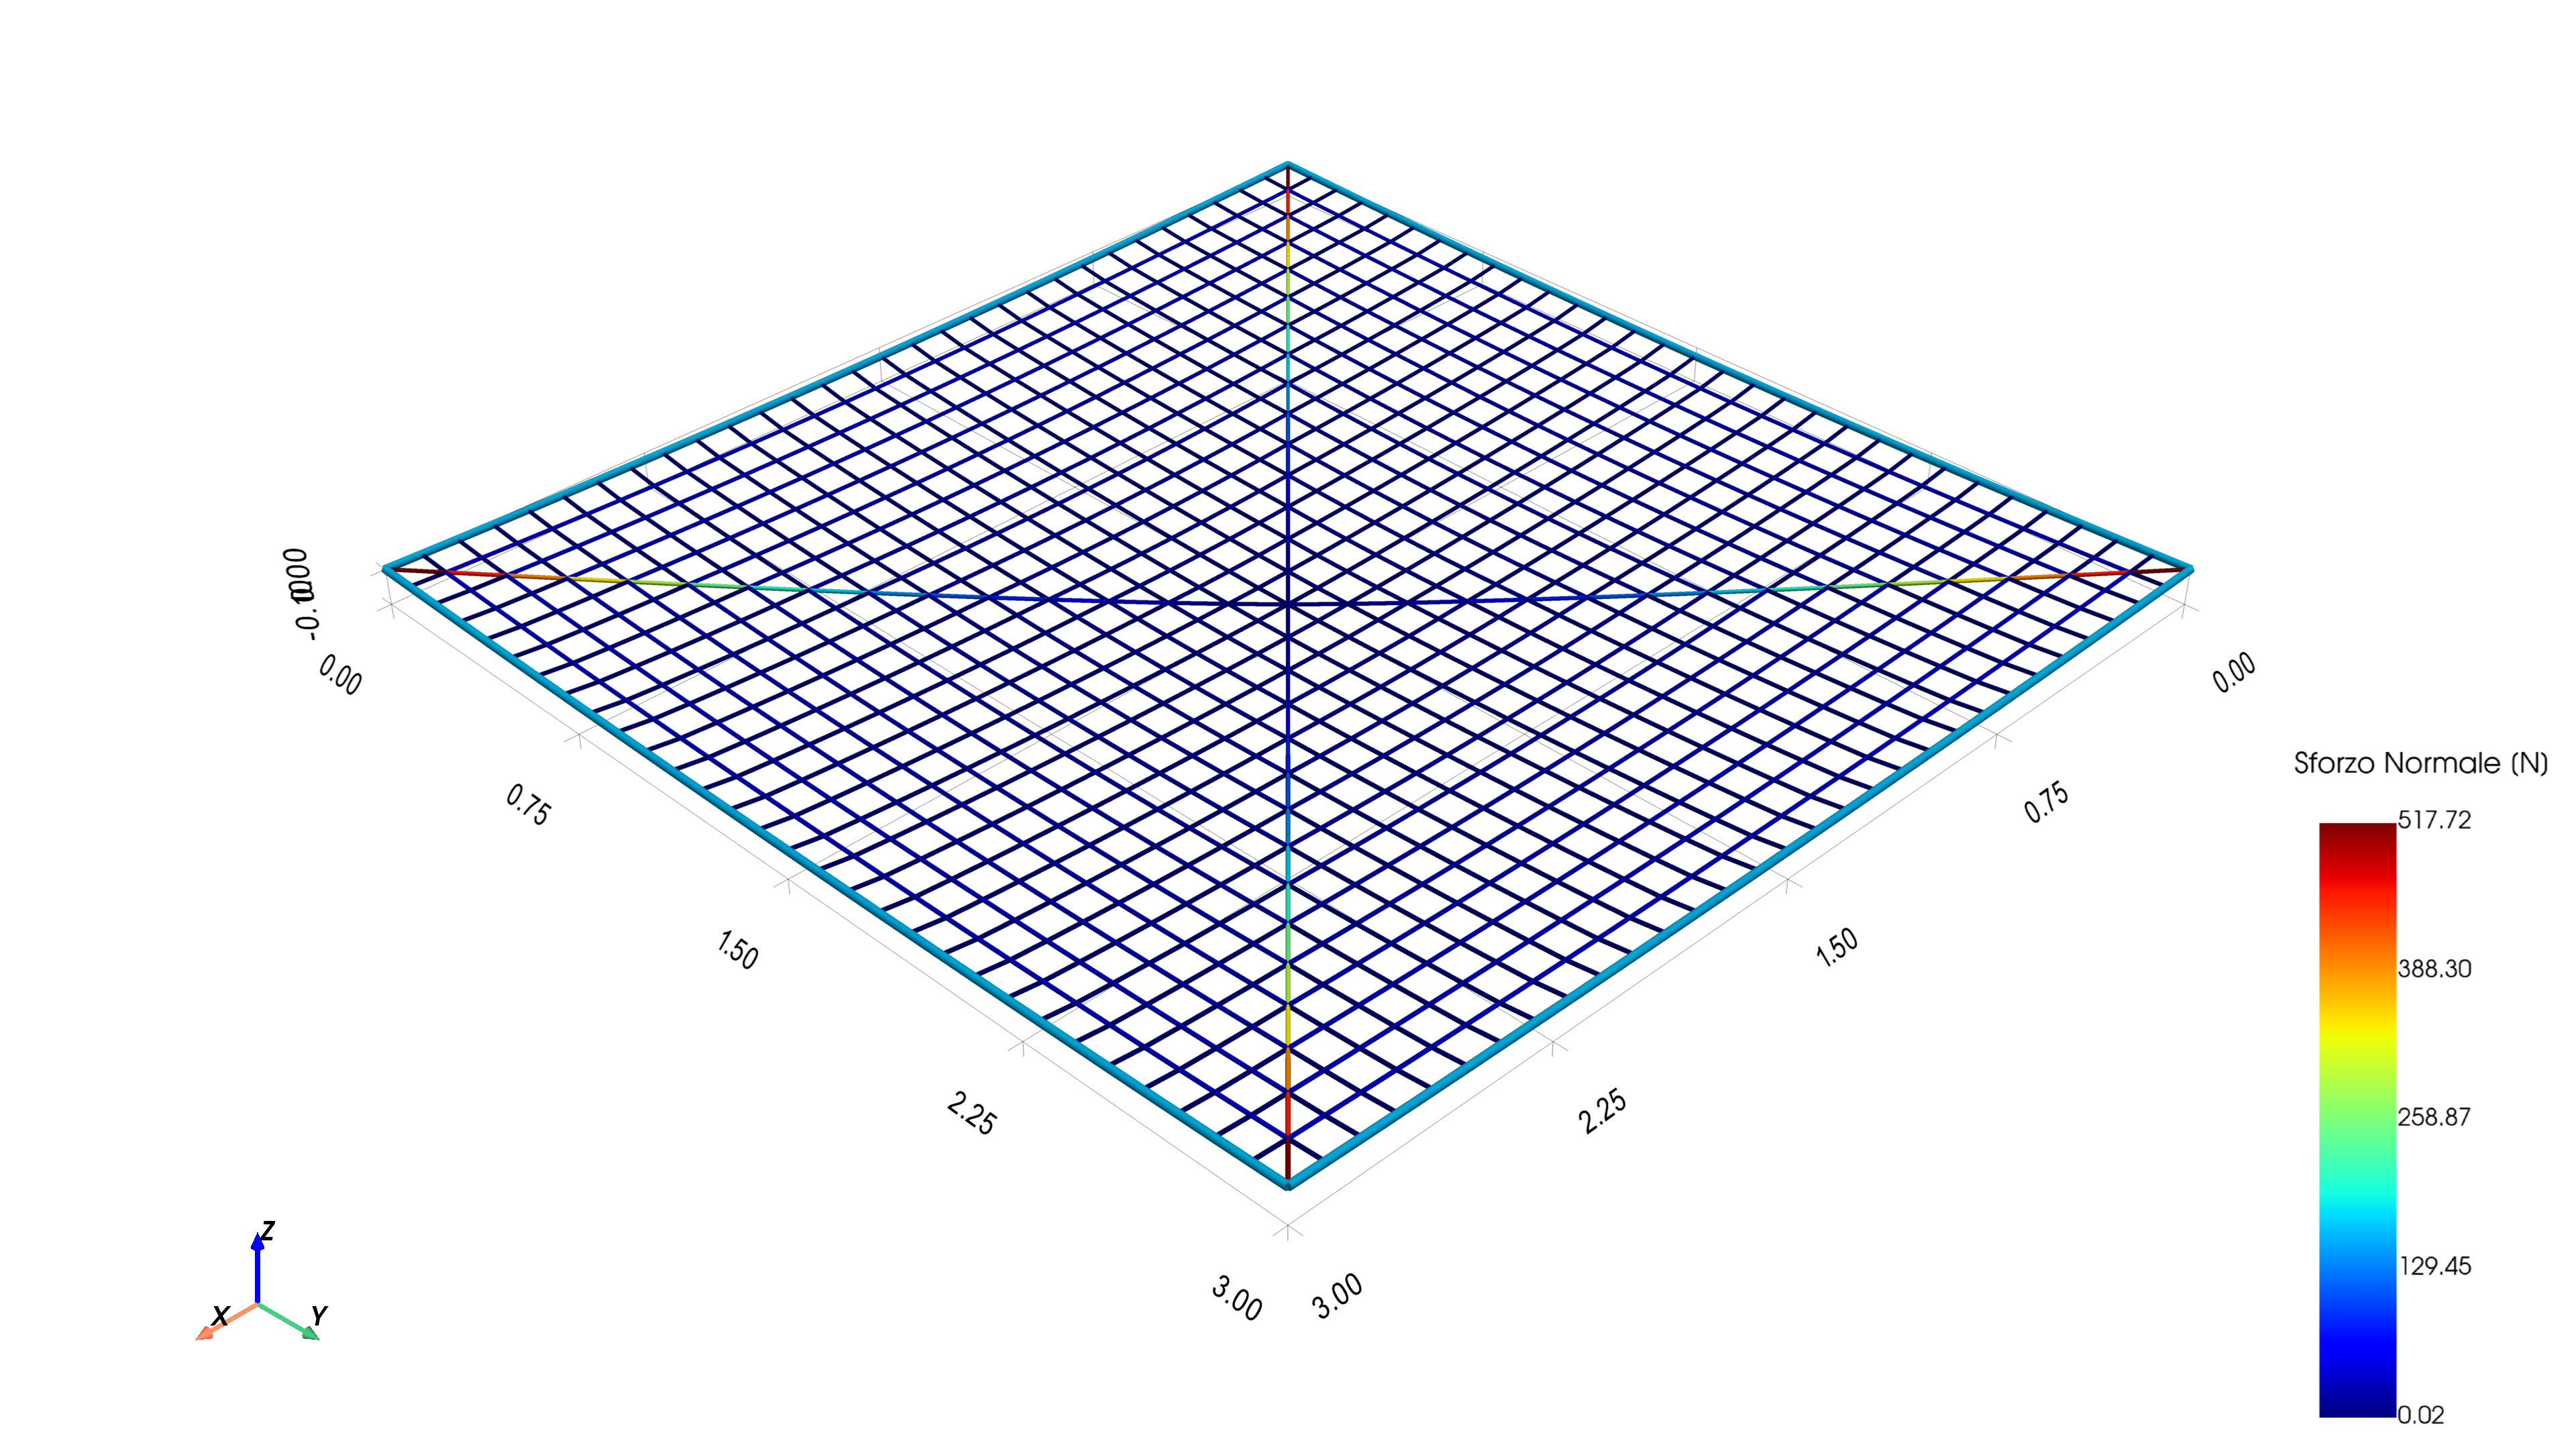
\includegraphics[width=\textwidth]{143_capitoli/capitolo4/immagini_capitolo_4/immagini_area/rete_aree_differenti1.png}
    \caption{Rete con configurazione differenziata a due vie}
    \label{fig:rete_aree_diffenti1}
\end{figure}

\begin{figure}[H]
    \centering
    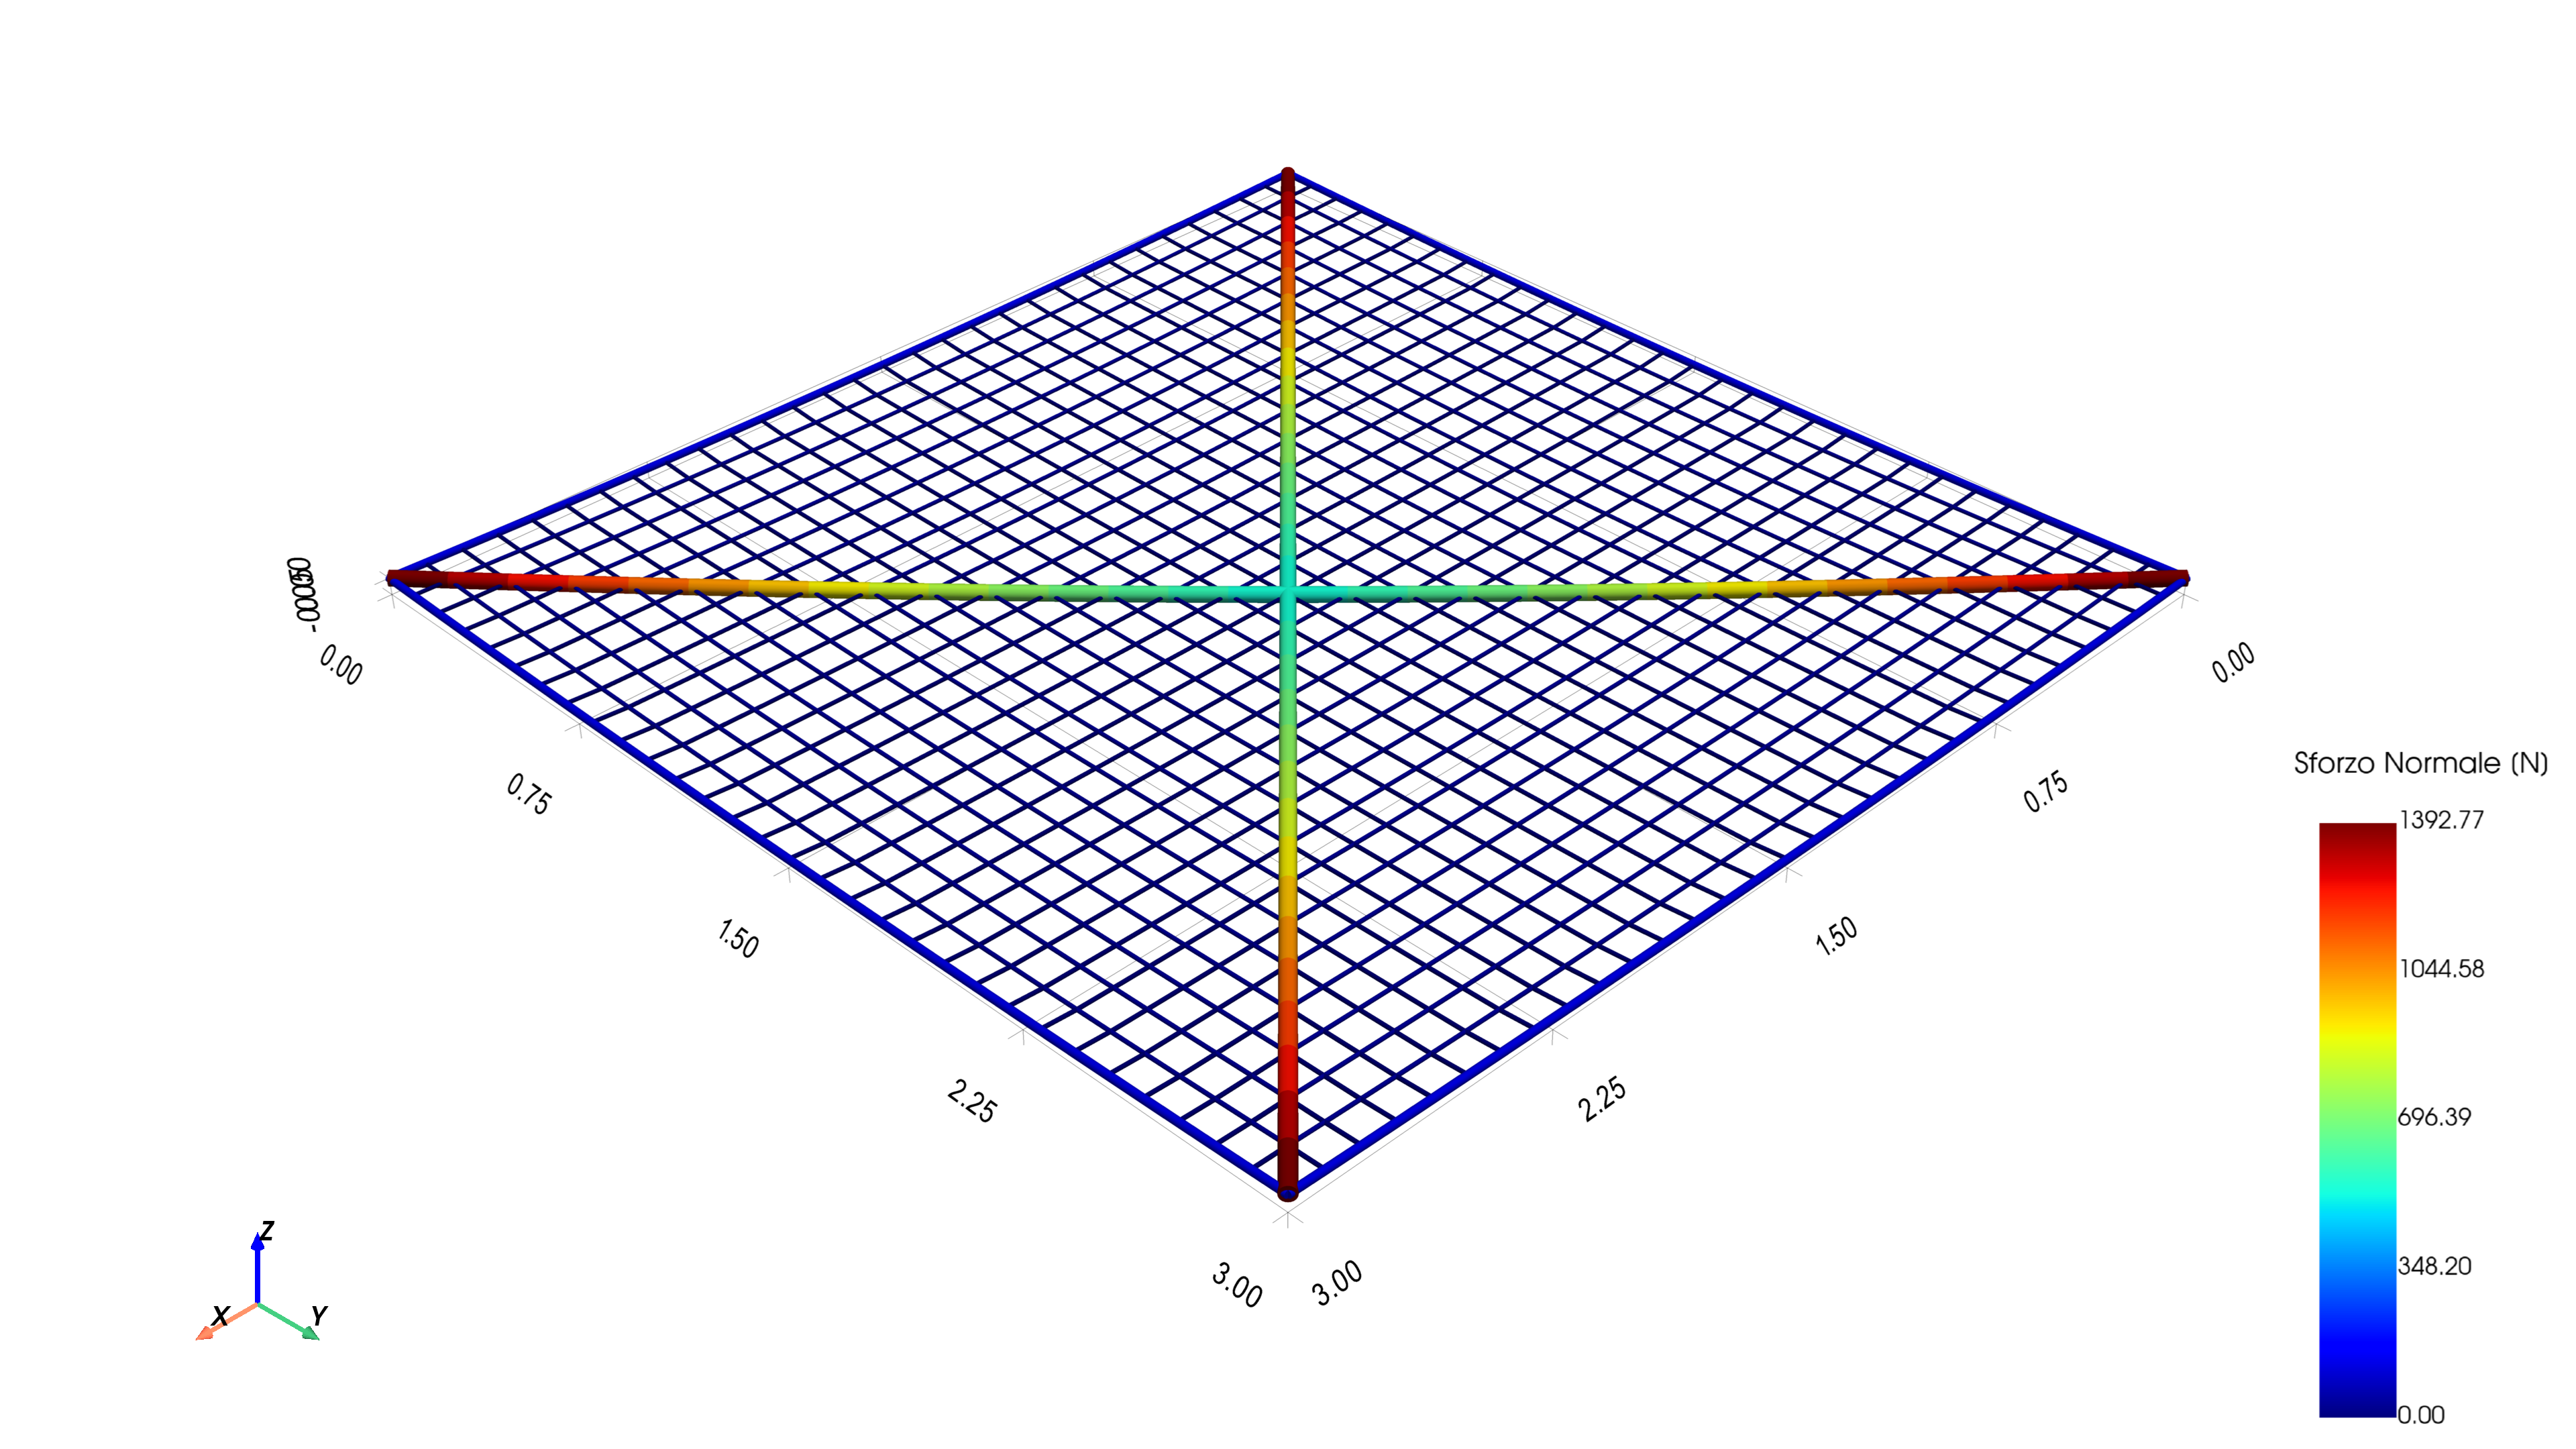
\includegraphics[width=\textwidth]{143_capitoli/capitolo4/immagini_capitolo_4/immagini_area/rete_aree_differenti2.png}
    \caption{Rete con configurazione differenziata a tre vie}
    \label{fig:rete_aree_differenti2}
\end{figure}

\begin{table}[htbp]
    \centering
    \caption{Proprietà geometriche e meccaniche della rete a maglia quadrata con funi di controvento - analisi di sensibilità alla rigidezza.}
    \vspace{5pt}
    \label{tab:caratteristiche_area_rete}
    \begin{tabularx}{\textwidth}{l c X}
        \hline
        \textbf{Parametro} & \textbf{Simbolo} & \textbf{Valore nominale} \\ \hline
        Dimensione totale della rete & $L_x \times L_y$ & $3.00 \times 3.00$ $[\text{m}]$ \\
        Dimensione della singola maglia & $l_{m_x} \times l_{m_y}$ & $10 \times 10$ $[\text{cm}]$ \\
        Diametro nominale delle funi & $\phi _1$ & $5.0$ $[\text{mm}]$ \\
        Diametro nominale delle funi & $\phi _2$ & $10.0$ $[\text{mm}]$ \\
        Modulo di elasticità longitudinale fune & $E$ & 2.1e9 $[\text{Pa}]$ \\
        Area della sezione trasversale fune & $A_1$ & 19.63 $[\text{mm}^2]$ \\
        Area della sezione trasversale fune & $A_2$ & 78.54 $[\text{mm}^2]$ \\
        Regolarizzazione del legame costitutivo & $\beta$ & 1e9 $[-]$\\
        Rapporto di laschezza in entrambe le direzioni & $\xi$ & 0 $[\text{\%}]$ \\ \hline
    \end{tabularx}
\end{table}

\subsection{Il fenomeno dello \textit{slack} nelle reti di cavi}
Nella trattazione della fune monodimensionale soggetta al peso proprio, qualora la lunghezza del suo sviluppo risulti superiore alla distanza lineare tra i vincoli di estremità, si definisce la condizione di fune \textit{lasca} o di \textit{slack}. In tale configurazione, la fune si trova in bando ed è caratterizzata da un tiro orizzontale poco significativo. 

In modo analogo, per sistemi discreti bidimensionali si utilizza la dicitura di rete lasca (\textit{net cables with slack}) per indicare una rete in cui lo sviluppo geometrico dei cavi costituenti è maggiore della distanza tra i vincoli perimetrali. Di conseguenza la rete non risulterà soggetta a tensioni elevate in direzione ortogonale a quella dei lati vincolati. Tuttavia, il caso in cui entrambi i lati della maglia siano più lunghi dei rispettivi lati vincolati introduce una complessità analitica e strutturale superiore rispetto al caso monodimensionale. 

Il fenomeno dello \textit{slack} si verifica in maniera differenziata in funzione della geometria della mesh assunta: 
\begin{itemize}
    \item \textbf{Rete a maglia quadrata (\textit{squared mesh} (Q)):} se lungo le direzioni principali dell'orditura ($x$ e $y$) lo stato tensionale è idealmente dominato da sforzi normali di trazione, lungo le direzioni inclinate gli sforzi di trazione generano sollecitazioni di taglio. Lungo le diagonali principali che uniscono gli angoli, perciò, avremo una sollecitazione di trazione massima, a cui corrisponde in direzione ortogonale una compressione. Come visibile dai risultati riportati in figura \cref{fig:rete_Q_slack}, si creano delle zone del dominio della rete in cui molti elementi vanno in \textit{slack} perchè compressi.
    \item \textbf{Rete a maglia romboidale (\textit{diamond mesh} (D)):} in questo caso, la maglia risulta ruotata di $45^\circ$ rispetto alla precedente. Di conseguenza la direzione in cui si verifica lo \textit{slack} è ortogonale rispetto al caso della mesh quadrata, come visibile in \cref{fig:rete_D_slack}. Assumendo un dominio in cui  $L_y = L_x = L$, le diagonali di lunghezza $\sqrt{2} L$ rappresentano le direzioni in cui si localizzano i maggiori allungamenti del dominio, inducendo l'allentamento dei cavi disposti lungo le direzioni evidenziate.
\end{itemize}

\begin{figure}[H]
   \centering
    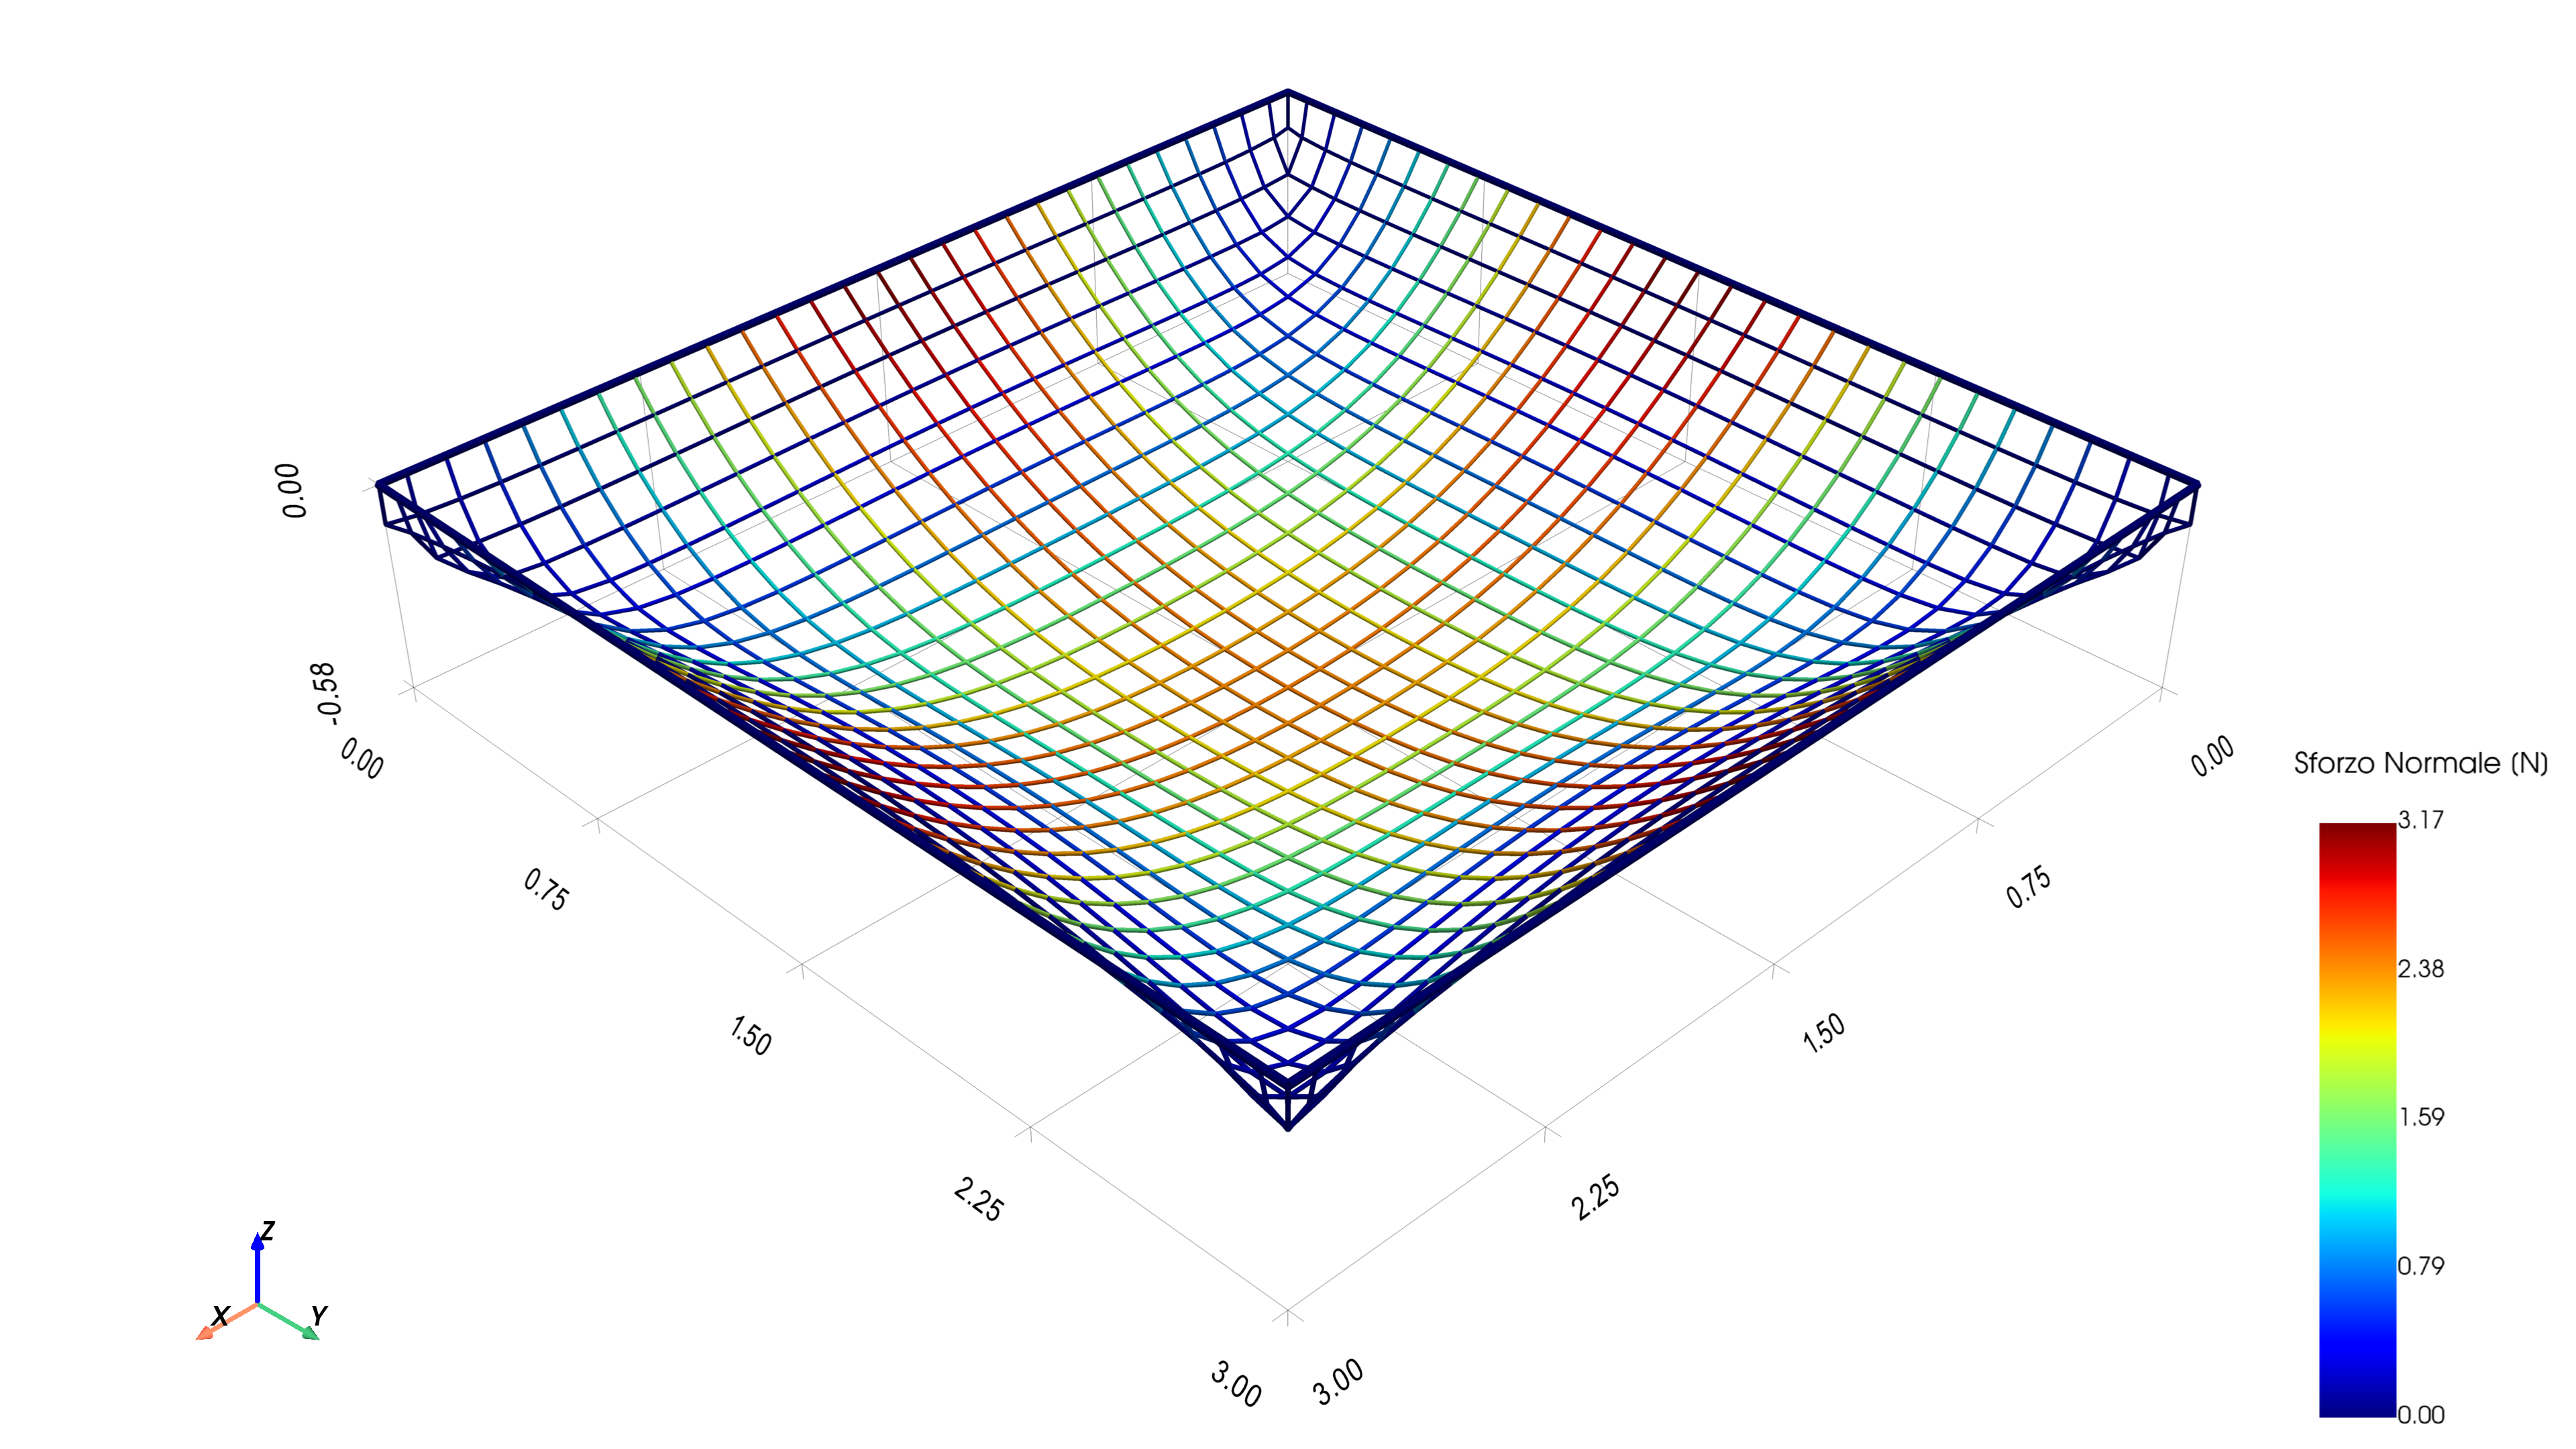
\includegraphics[width=\textwidth]{143_capitoli/capitolo4/immagini_capitolo_4/immagini_slack/rete_Q_slack.png}
    \caption{Rete a maglia quadrata in condizione di slack}
    \label{fig:rete_Q_slack}
\end{figure}

\begin{figure}[H]
   \centering
    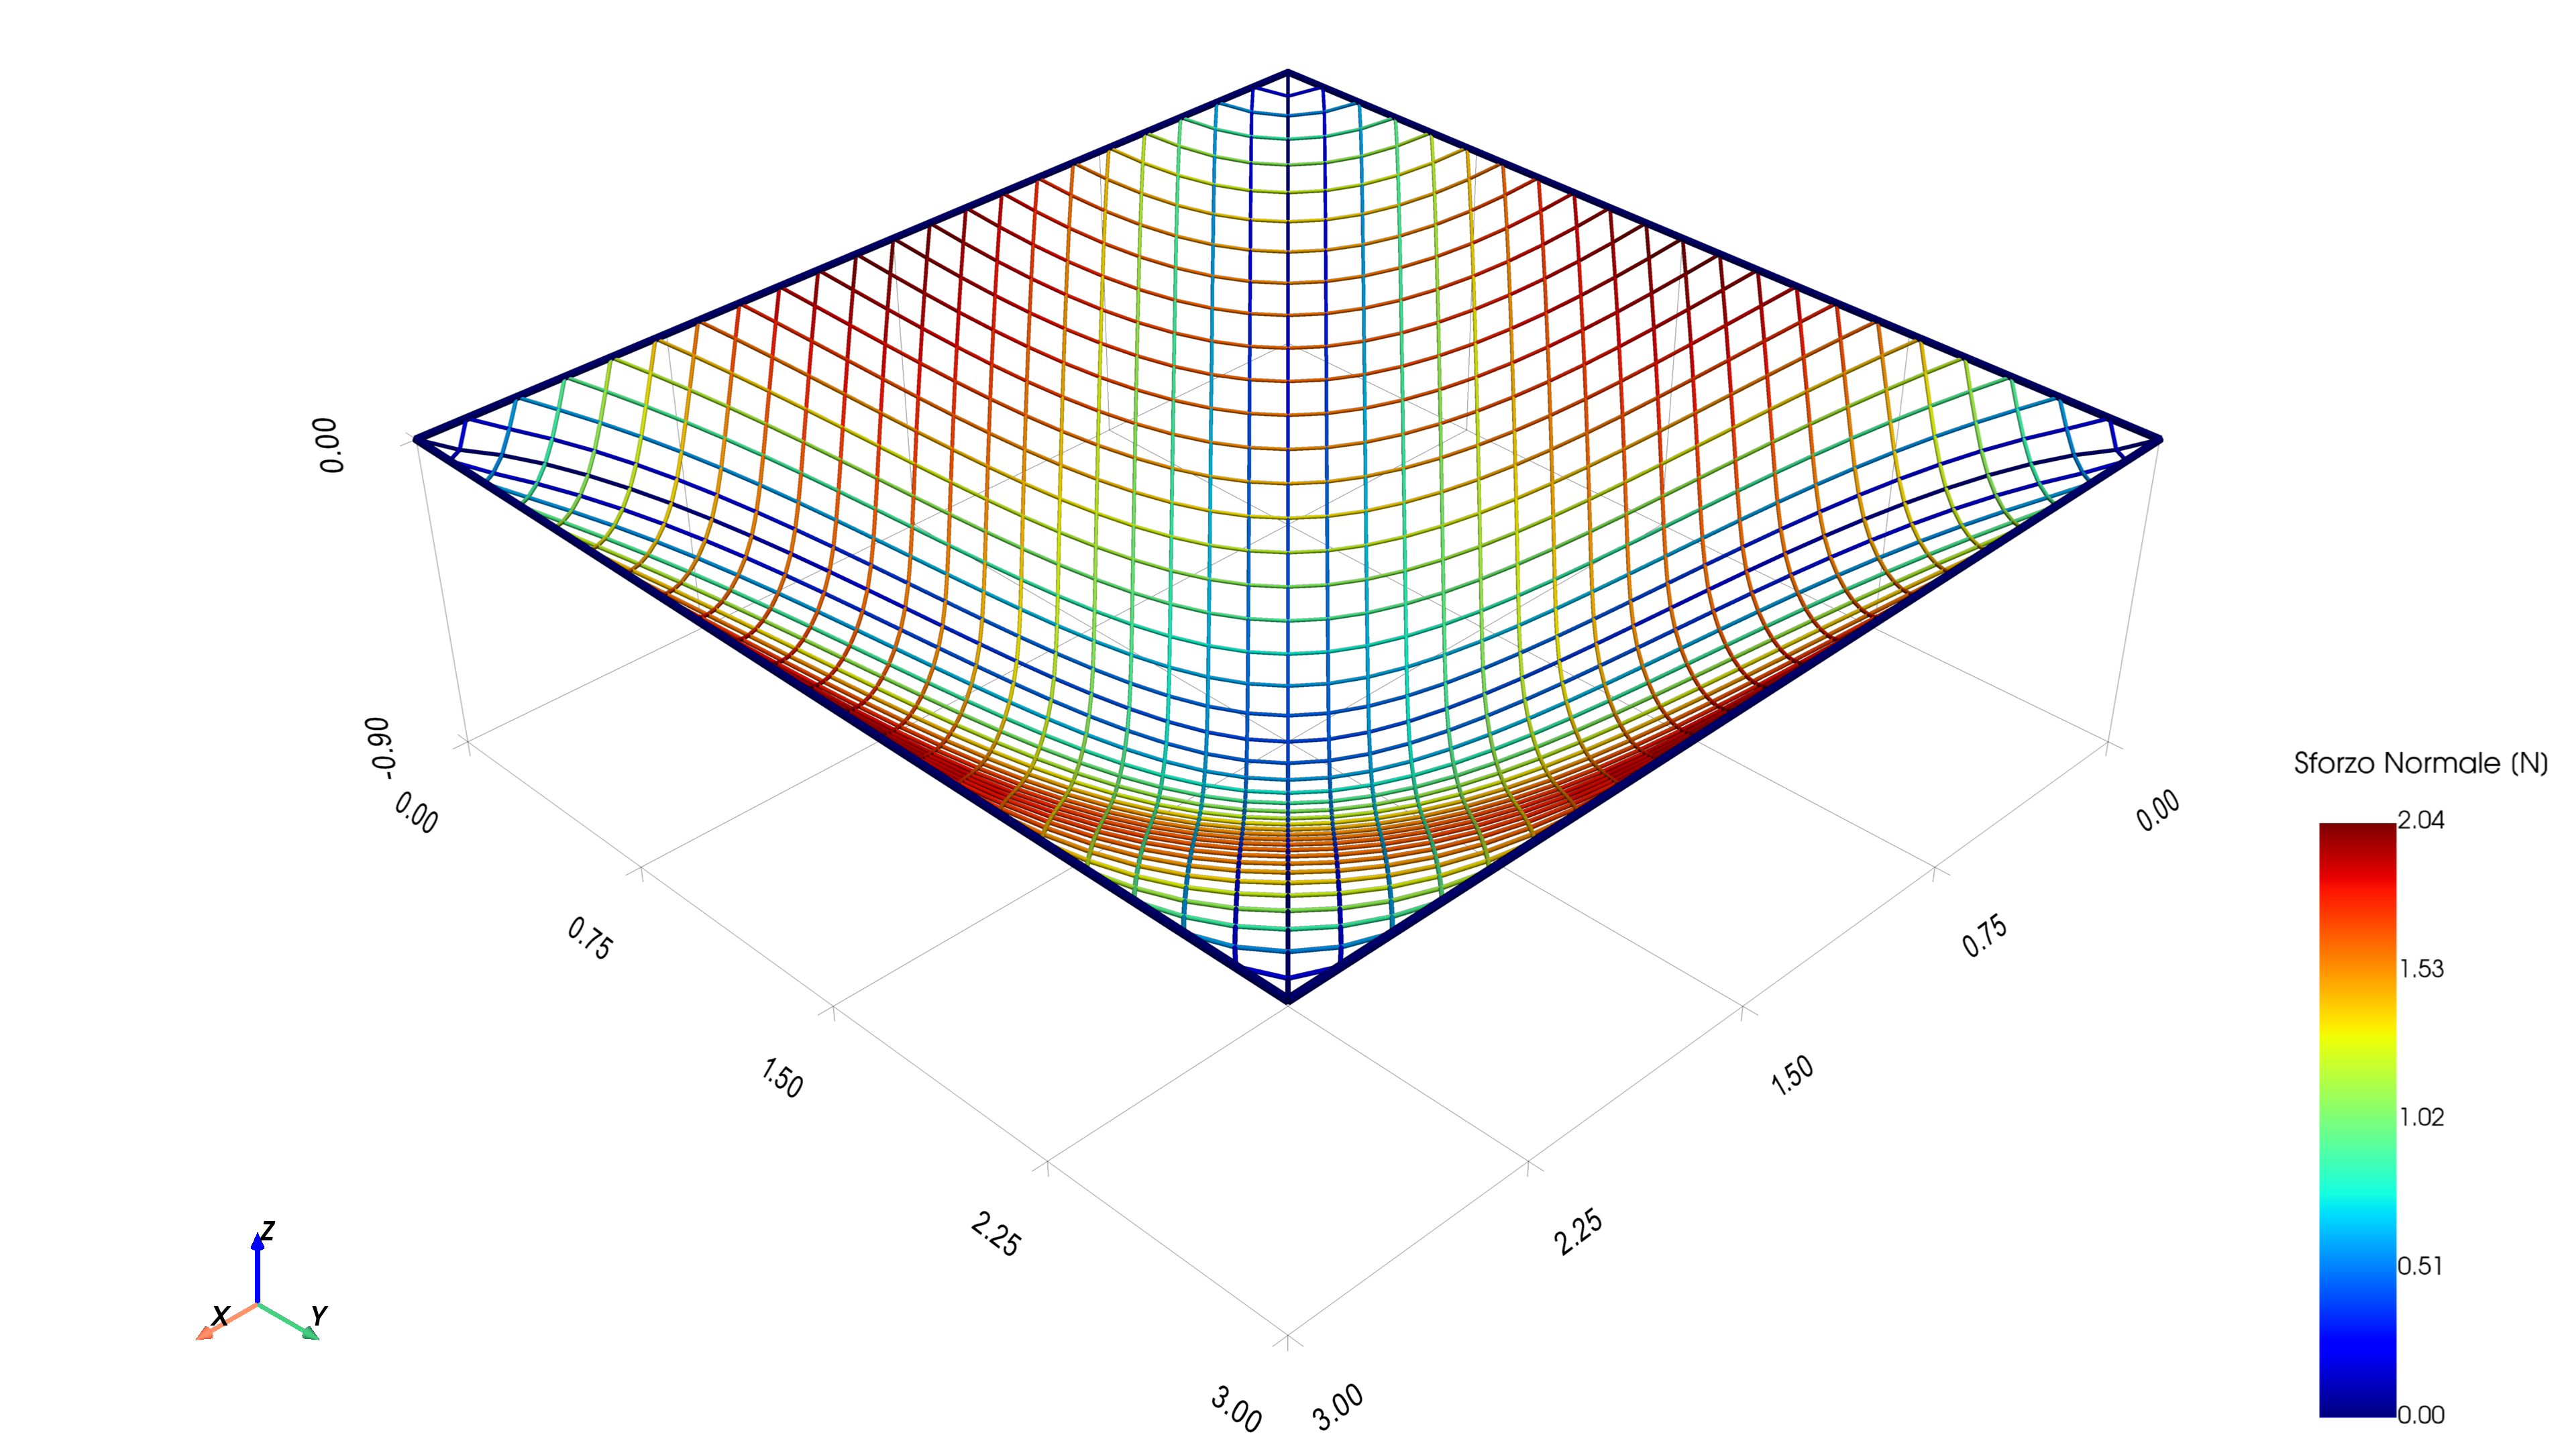
\includegraphics[width=\textwidth]{143_capitoli/capitolo4/immagini_capitolo_4/immagini_slack/rete_D_slack.png}
    \caption{Rete a maglia romboidale in condizione di slack}
    \label{fig:rete_D_slack}
\end{figure}

\begin{table}[htbp]
    \centering
    \caption{Proprietà geometriche e meccaniche delle reti di funi di \cref{fig:rete_Q_slack,fig:rete_D_slack}}
    \vspace{5pt}
    \label{tab:caratteristiche_reti_cap_slack}
    \begin{tabularx}{\textwidth}{l c X}
        \hline
        \textbf{Parametro} & \textbf{Simbolo} & \textbf{Valore nominale} \\ \hline
        Dimensione totale della rete & $L_x \times L_y$ & $3.00 \times 3.00$ $[\text{m}]$ \\
        Dimensione della singola maglia (Q) & $l_{m_x} \times l_{m_y}$ & $10 \times 10$ $[\text{cm}]$ \\
        Dimensione della singola maglia (D) & $l_{m_x} \times l_{m_y}$ & $9.64 \times 9.64$ $[\text{cm}]$ \\
        Diametro nominale delle funi di maglia & $\phi _1$ & $5.0$ $[\text{mm}]$ \\
        Diametro nominale delle funi di bordo & $\phi _2$ & $10.0$ $[\text{mm}]$ \\
        Area sezione trasversale fune di maglia & $A_1$ & 19.63 $[\text{mm}^2]$ \\
        Area sezione trasversale fune di bordo & $A_2$ & 78.54 $[\text{mm}^2]$ \\
        Modulo di elasticità longitudinale fune & $E$ & 2.1e9 $[\text{Pa}]$ \\
        Regolarizzazione del legame costitutivo & $\beta$ & 1e9 $[-]$\\
        Rapporto di laschezza (Q) in entrambe le direzioni & $\xi_Q$ & 10 $[\%]$\\
        Rapporto di laschezza (D) in entrambe le direzioni & $\xi_D$ & 10 $[\%]$\\ \hline
    \end{tabularx}
\end{table}

Questo comportamento discreto trova un parallelo continuo nel campo delle membrane e delle piastre sottili, dove l'insorgere della compressione diagonale provoca un instabilità flessionale fuori dal piano che si manifesta con la formazione di "rughe" parallele alla direzione di trazione principale. In entrambe i sistemi, la struttura modifica la propria topologia tridimensionale attraverso spostamenti fuori dal piano al fine di annullare la compressione interna e minimizzare l'energia potenziale totale del sistema.

Dal punto di vista numerico, l'insorgere dello \textit{slack} comporta l'annullamento delle rigidezza e della tensione di ampie porzioni della rete. L'assenza di resistenza a compressione dell'elemento fune genera la comparsa di moti rigidi ad energia nulla (cinematismi locali). Di conseguenza la matrice di rigidezza tangente globale del sistema diventa singolare (o quasi-singolare) compromettendo inevitabilmente la convergenza dell'algoritmo di soluzione. Per superare questa limitazione computazionale e restituire unicità alla soluzione numerica, si ricorre principalmente a due strategie: 

\begin{itemize}
   \item \textbf{Analisi dinamica:} anzichè risolvere il problema statico di un sistema labile (cinematismo), si formula un problema dinamico equivalente introducendo le forze d'inerzia ed uno smorzamento. L'equazione del moto assume la forma vista in \cref{eq:equilibrio_dinamico_problema}, dove $\underline{p}$ in tal caso è sostituito dal vettore globale delle forze peso definito in \cref{eq:vettore_peso}. Imponendo delle condizioni iniziali ($\underline{x}_0$ e $\underline{\dot x}_0$) arbitrarie e diverse da zero, il sistema viene lasciato oscillare sotto l'azione del peso proprio fino a quando lo smorzamento non dissipa l'energia cinetica, conducendo la rete ad una configurazione di equilibrio statico finale.
   
   Dal punto di vista computazionale, l'impiego dell'analisi dinamica svincola la risoluzione del problema aggirando la singolarità della matrice globale di rigidezza tangente $T(\underline{x})$: lo schema esplicito richiede infatti l'inversione della sola matrice di massa globale, che essendo diagonale e definita positiva, rimane sempre invertibile.
   \item \textbf{Regolarizzazione della legge costitutiva:} uno stratagemma numerico utilizzato nei solutori statici consiste nell'evitare che tensione e modulo elastico dell'elemento fune si annullino completamente in compressione. Si introduce una legge costitutiva modificata per la quale, quando il cavo subisce un accorciamento, lo sforzo ed il modulo elastico non scendono a zero ma si stabilizzano su valori infinitesimi positivi (nel nostro caso si è assunto $\sigma \approx 1Pa$ e $E_{eff} \approx 1e^{-2}Pa$). Questa minima rigidezza residua elimina i moti rigidi ad energia nulla ed impedisce alla matrice di rigidezza di diventare singolare, garantendo la convergenza dell'algoritmo di Newton-Raphson e preservando l'aderenza fisica del modello, in quanto lo sforzo residuo calcolato risulta strutturalmente trascurabile.
\end{itemize}

\subsubsection{Regolarizzazione del legame costitutivo}
Come analizzato in precedenza, il modello costitutivo ideale per un elemento fune in campo elastico, a causa della sua incapacità di sopportare sforzi di compressione, è il modello unilatero denominato \textit{tension-only}. Nella formulazione riportata in \cref{eq:tension_only2}, tale comportamento viene descritto da una funzione bilineare a tratti.

Tuttavia, l'utilizzo di una funzione a tratti presenta un punto in corrispindenza dell'origine in cui la funzione non risulta derivabile. Gli algoritmi di risoluzione come il metodo di Newton-Raphson, mostrano difficoltà di convergenza in presenza di relazioni costitutive non derivabili, a causa delle brusche oscillazioni della rigidezza tangente nei punti di transizione. 

Per superare tale limitazione computazionale e favorire la convergenza numerica nel calcolo delle reti lasche si è adottata la regolarizzazione della legge costitutiva. Nello specifico, la relazione bilineare viene approssimata tramite una funzione derivabile su tutto il suo dominio $(e_{11} \in [-\infty, \infty])$. La relazione costitutiva regolarizzata assume pertanto la forma:
\begin{equation}
   \sigma = \sigma_{min} + \frac{E}{\beta} \ln\left( 1 + e^{\beta e_{11}} \right) 
   \label{eq:bilinear_smooth}
\end{equation}

dove: 
\begin{itemize}
   \item $E$ rappresenta il modulo elastico del materiale nel tratto teso;
   \item $e_{11}$ è la componente assiale del tensore di deformazione di Green-Lagrange;
   \item $\sigma_{min}$ è il valore di tensione minima residua;
   \item $\beta$ è un parametro di regolarizzazione adimensionale che governa la transizione tra il comportamento lasco e quello teso.
\end{itemize}

La scelta del parametro $\beta$ rappresenta un compromesso di fondamentale importanza: l'impiego di valori di $\beta$ elevati consente di approssimare con estrema fedeltà la legge bilineare ideale, ma introduce gradienti che penalizzano la stabilità dell'algoritmo di soluzione. Al contrario, valori di $\beta$ contenuti migliorano significativamente la convergenza a discapito, però, della rispondenza fisica del modello nell'intorno del punto in cui $e_{11} \approx 0$. Per tali ragioni, unitamente alle soluzioni presentate, vengono fornite le informazioni riguardanti il legame costitutivo adottato (\textit{tension-only} puro o regolarizzato) e, nel secondo caso, il valore del parametro $\beta$ impiegato.

Come mostrato in \cref{fig:legame_regolarizzato_sigma,fig:legame_regolarizzato_E}, la formulazione regolarizzata descritta dall'\cref{eq:bilinear_smooth} riprende fedelmente l'andamento della legge \textit{tension-only} classica, garantendo al contempo la continuità della derivata prima su tutto il dominio di definizione. 
\begin{figure}[H]
   \centering
    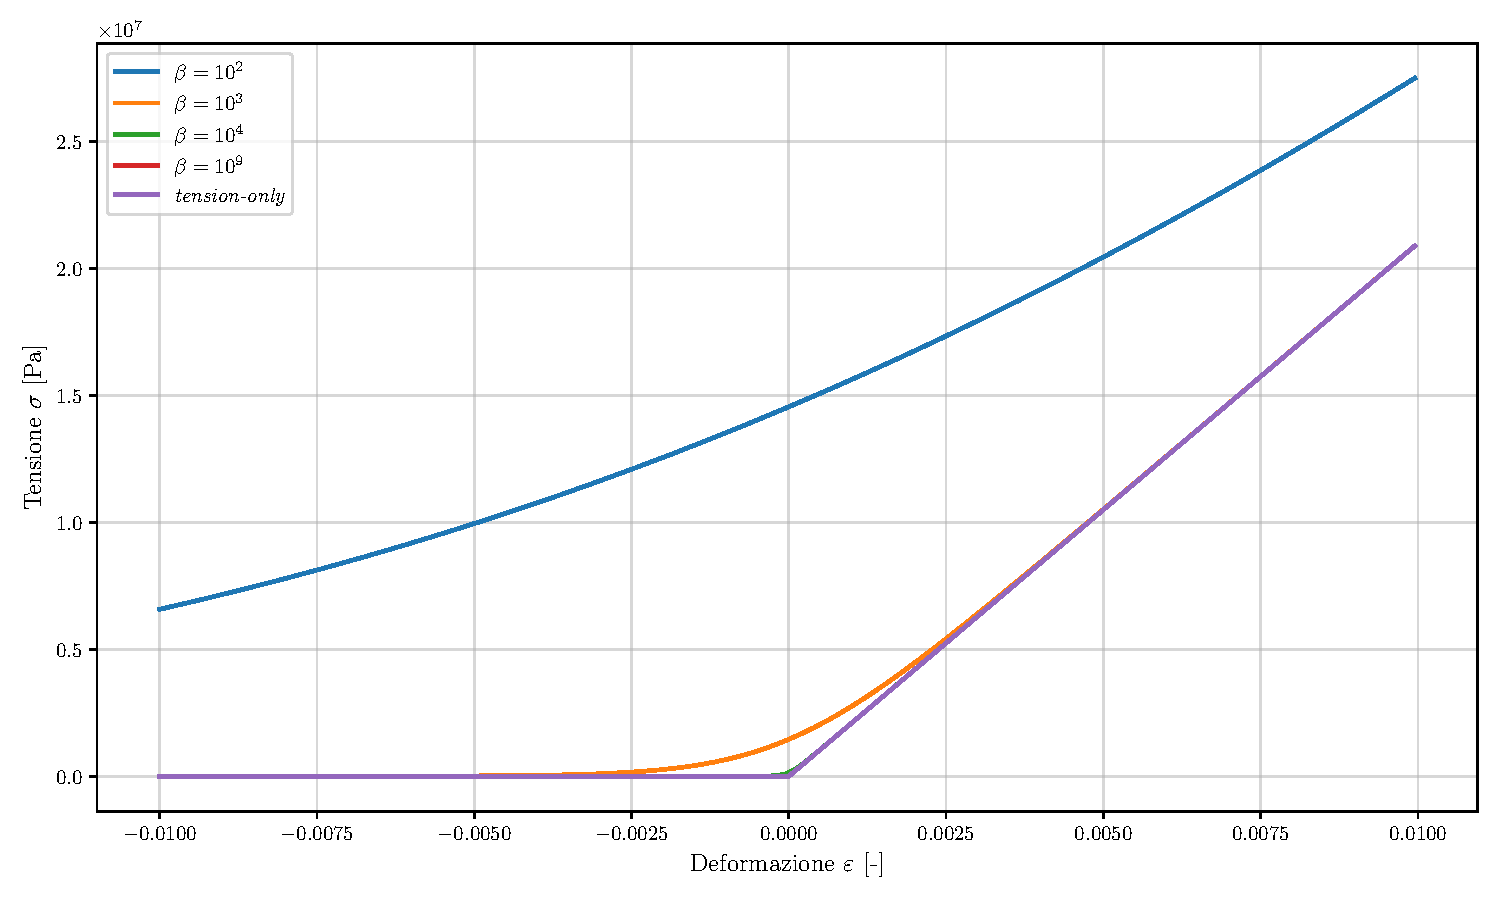
\includegraphics[width=\textwidth]{143_capitoli/capitolo4/immagini_capitolo_4/immagini_slack/Legame_regolarizzato_sigma.pdf}
    \caption{Legame costitutivo regolarizzato $\sigma - \varepsilon$}
    \label{fig:legame_regolarizzato_sigma}
\end{figure}

\begin{figure}[H]
   \centering
    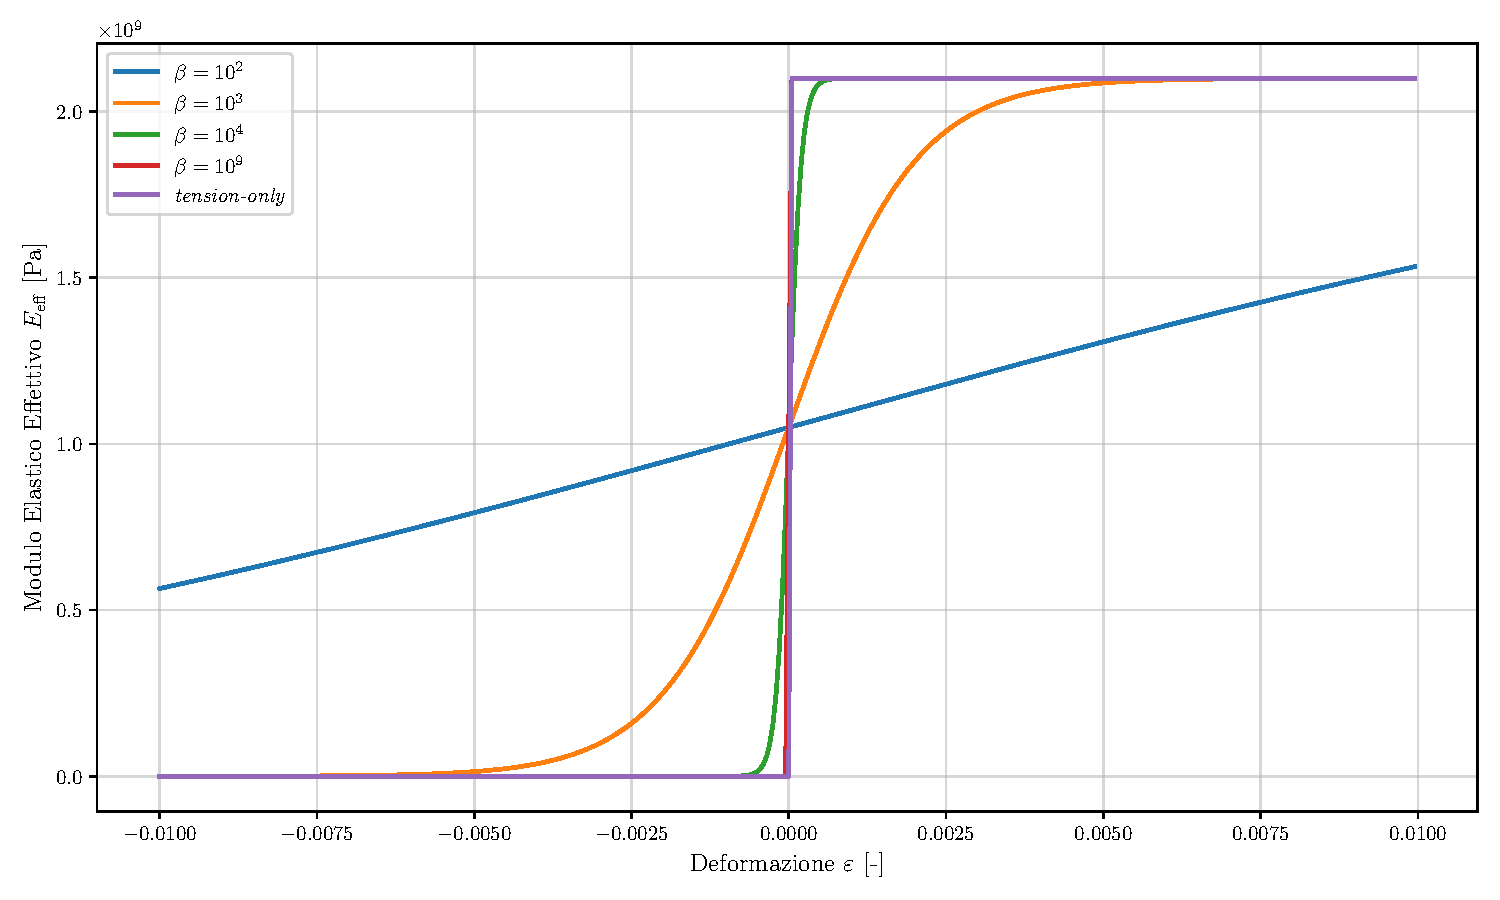
\includegraphics[width=\textwidth]{143_capitoli/capitolo4/immagini_capitolo_4/immagini_slack/Legame_regolarizzato_E.pdf}
    \caption{Legame costitutivo regolarizzato $E_{\mathrm{eff}} - \varepsilon$}
    \label{fig:legame_regolarizzato_E}
\end{figure}

\subsubsection{Laschezza della rete}
La valutazione della freccia massima (\textit{sag}) al variare dello sviluppo lineare della rete rispetto alla distanza tra i vincoli può essere espressa quantitativamente tramite i valori del \textit{rapporto di laschezza} (o \textit{slackness ratio}) lungo le due direzioni principali della rete $\xi_x$ e $\xi_y$, definiti coerentemente con l'\cref{eq:rapporto_laschezza} espressa in pecentuale. 

Al fine di stimare l'entità della freccia iniziale e garantire il rispetto delle prescrizioni geometriche imposte dalla normativa EN 1263-1 \cite{EN1263-1} per la prova statica di assorbimento di energia, si è condotta un'analisi parametrica su una rete di dimensioni nominali pari a $3\, \text{m} \times 3\,\text{m}$ (come previsto dalla norma per la stessa prova), ipotizzando un medesimo valore di \textit{rapporto di laschezza} lungo entrambe le direzioni principali ($\xi_x = \xi_y = \xi$). Nello specifico, è stata determinata la curva caratteristica che correla $\xi$ al valore della freccia massima $f$ risultante.

I risultati dell'analisi parametrica per la configurazione a maglia quadrata (Q) e per quella romboidale (D) sono illustrati rispettivamente in \cref{fig:diagramma_sag_Q} e in \cref{fig:diagramma_sag_D}.

I parametri geometrici e meccanici adottati nei modelli numerici per la generazione delle curve $f - \xi$ sono riassunti in \cref{tab:caratteristiche_reti_slack_ratio}.
\begin{figure}[H]
   \centering
    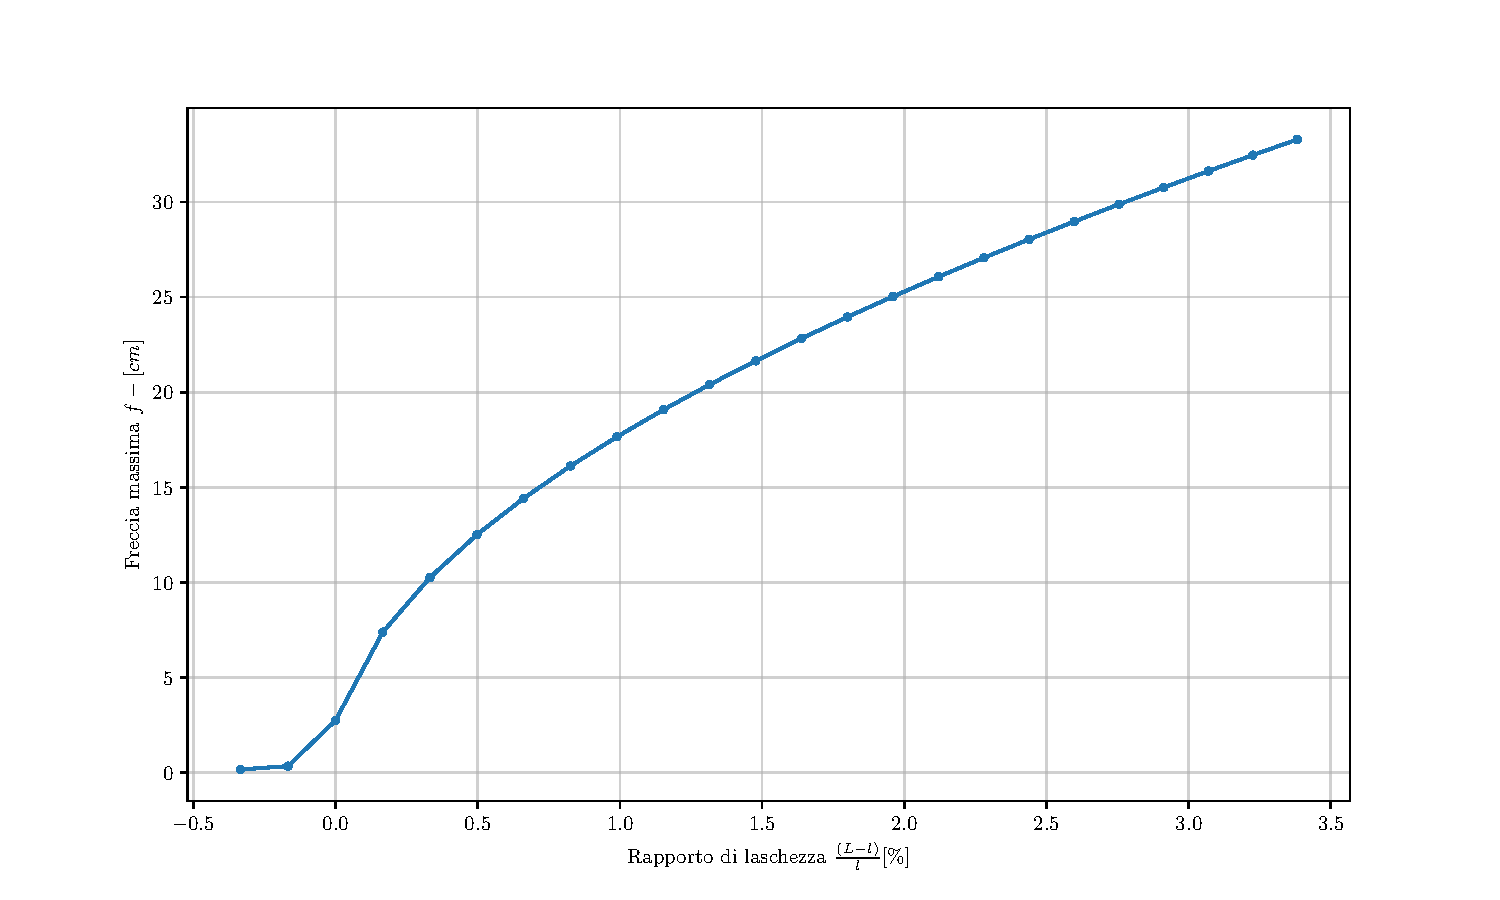
\includegraphics[width=\textwidth]{143_capitoli/capitolo4/immagini_capitolo_4/immagini_slack/grafico_Q.pdf}
    \caption{Diagramma \textit{sag} - \textit{slackness ratio} per una rete a maglia quadrata}
    \label{fig:diagramma_sag_Q}
\end{figure}

\begin{figure}[H]
   \centering
    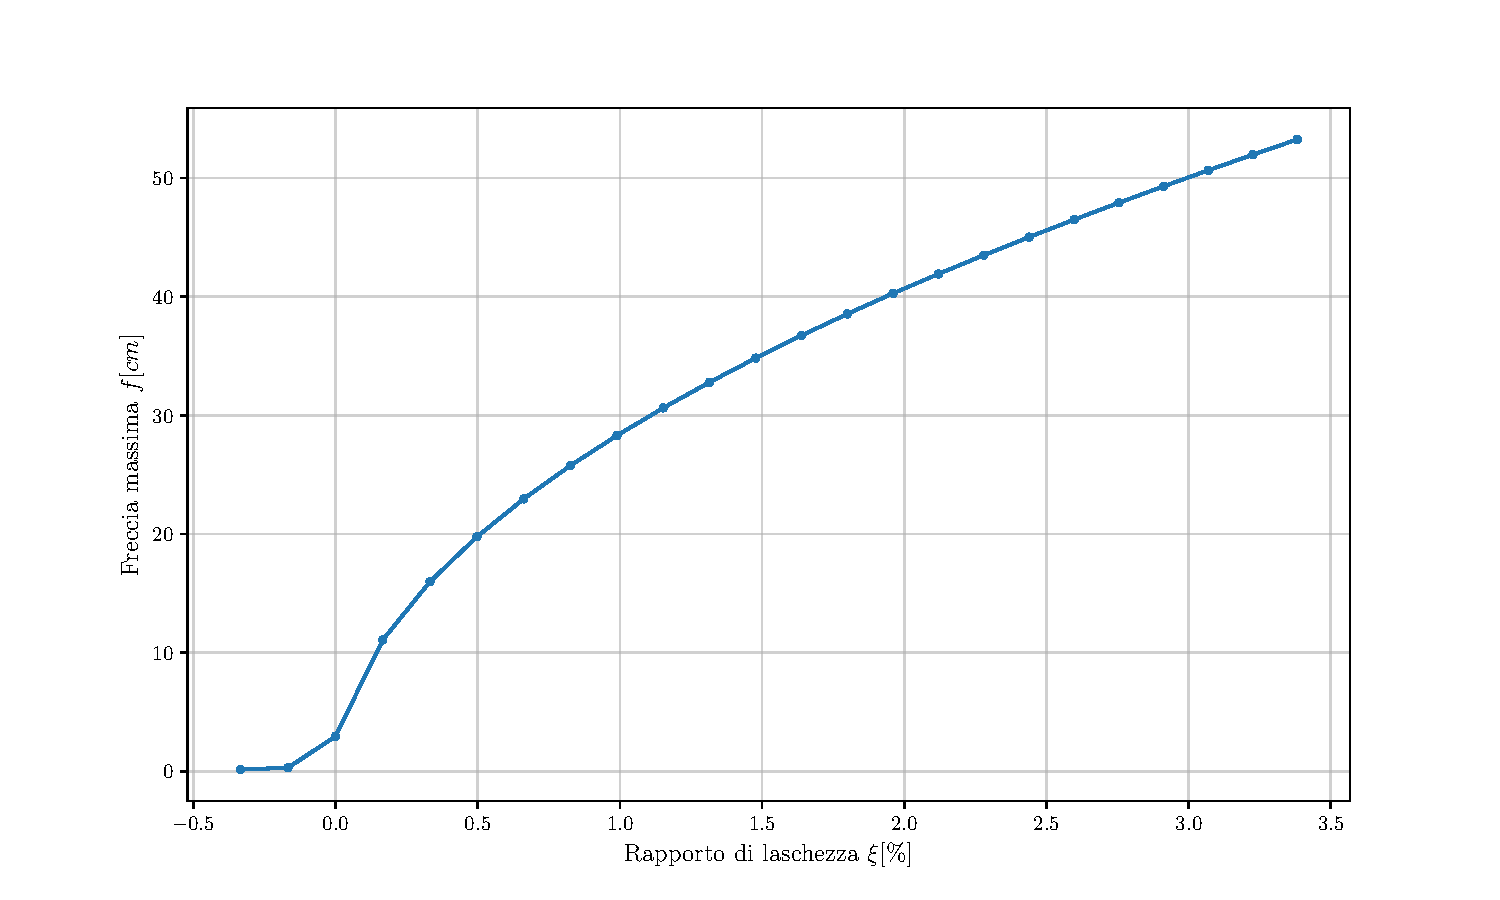
\includegraphics[width=\textwidth]{143_capitoli/capitolo4/immagini_capitolo_4/immagini_slack/grafico_D.pdf}
    \caption{Diagramma \textit{sag} - \textit{slackness ratio} per una rete a maglia romboidale}
    \label{fig:diagramma_sag_D}
\end{figure}

\begin{table}[htbp]
    \centering
    \caption{Proprietà geometriche e meccaniche delle reti impiegate per la determinazione dei diagrammi di \cref{fig:diagramma_sag_Q,fig:diagramma_sag_D}}
    \vspace{5pt}
    \label{tab:caratteristiche_reti_slack_ratio}
    \begin{tabularx}{\textwidth}{l c X}
        \hline
        \textbf{Parametro} & \textbf{Simbolo} & \textbf{Valore nominale} \\ \hline
        Dimensione totale della rete & $L_x \times L_y$ & $3.00 \times 3.00$ $[\text{m}]$ \\
        Dimensione della singola maglia (Q) & $l_{m_x} \times l_{m_y}$ & $10 \times 10$ $[\text{cm}]$ \\
        Dimensione della singola maglia (D) & $l_{m_x} \times l_{m_y}$ & $9.64 \times 9.64$ $[\text{cm}]$ \\
        Diametro nominale delle funi di maglia & $\phi _1$ & $5.0$ $[\text{mm}]$ \\
        Area della sezione trasversale fune & $A_1$ & 19.63 $[\text{mm}^2]$ \\ 
        Modulo di elasticità longitudinale fune & $E$ & 2.1e9 $[\text{Pa}]$ \\
        Regolarizzazione del legame costitutivo & $\beta$ & 1e9 $[-]$\\ \hline
    \end{tabularx}
\end{table}

È importante sottolineare come i due grafici non risultino direttamente confrontabili in termini di rigidezza nei confronti dei carichi verticali. Infatti, per garantire le medesime dimensioni complessive della rete, la dimensione della singola maglia nella configurazione romboidale differisce da quella della maglia quadrata per un fattore pari a $\sqrt{2}$, comportando di conseguenza un diverso numero complessivo di elementi costitutivi nei due modelli.

Dai grafici è possibile quindi risalire ai valori del rapporto di laschezza $\xi$ (e, di conseguenza, alle tolleranze sulla lunghezza), affinchè la freccia della rete in configurazione di prova rispetti i limiti imposti dalla normativa ($f = 5 \pm 1\, \text{cm}$). In particolare, per i casi analizzati, il rapporto di laschezza dovrà essere compreso tra $ 0.08\% < \xi_{Q} < 0.12\%$ per la geometria quadrata e tra $ 0.04\% < \xi_{D} < 0.07\%$ per quella romboidale.    

Dall'esame degli andamenti si evince che la tolleranza teorica sulla lunghezza dei lati della rete in esame dovrebbe essere confinata entro limiti estremamente stringenti al fine di scongiurare un'eccessiva deformabilità o, al contrario, uno stato di coazione iniziale indesiderato. Tuttavia, considerando le ordinarie tolleranze di fabbricazione e posa delle reti di sicurezza, risulta nella pratica industriale pressoché impossibile garantire uno scarto dimensionale contenuto entro frazioni di punto percentuale. Di conseguenza, nel contesto operativo reale, la conformità geometrica della rete non viene valutata tramite il controllo dimensionale preventivo dello sviluppo dei cavi, bensì verificando direttamente il valore della freccia residua $f$ mediante prove prestazionali di tipo passa / non passa.

\subsection{Comportamento sotto carichi concentrati}
Fino ad ora l'analisi numerica si è concentrata esclusivamente sulla configurazione di equilibrio della rete soggetta al solo peso proprio; nello specifico, nell'\cref{eq:problema_statico} si è assunto che il vettore dei carichi esterni fosse pari a: 
\begin{equation}
   \underline{f}_{ext} = \underline{f}_{g,e}
\end{equation}

Tuttavia, l'algoritmo implementato consente di estendere la trattazione includendo l'applicazione di forze concentrate, caratterizzate da intensità e direzioni arbitrarie, agenti su nodi specifici della mesh. In questo scenario, l'espressione del vettore dei carichi esterni si specifica per mezzo della relazione:
\begin{equation}
   \underline{f}_{ext} = \underline{f}_{g,e} + \underline{f}_{concentrate} 
\end{equation}

Ulteriori sviluppi e applicazioni del codice potranno prevedere l'implementazione di combinazioni lineari di vettori di forze concentrate. Tale approccio consentirà di simulare, in forma discretizzata, distribuizioni di carico continue in funzione delle esigenze dell'utente.

A scopo dimostrativo, nelle \cref{fig:forza_concentrata_verticale,fig:forza_concentrata_inclinata} viene illustrata la configurazione deformata e lo stato tensionale della rete ottenuti applicando una forza concentrata in corrispondenza del nodo di mezzeria. 

Le caratteristiche della rete analizzata e delle forze applicate sono riportate in 

\begin{figure}[H]
   \centering
    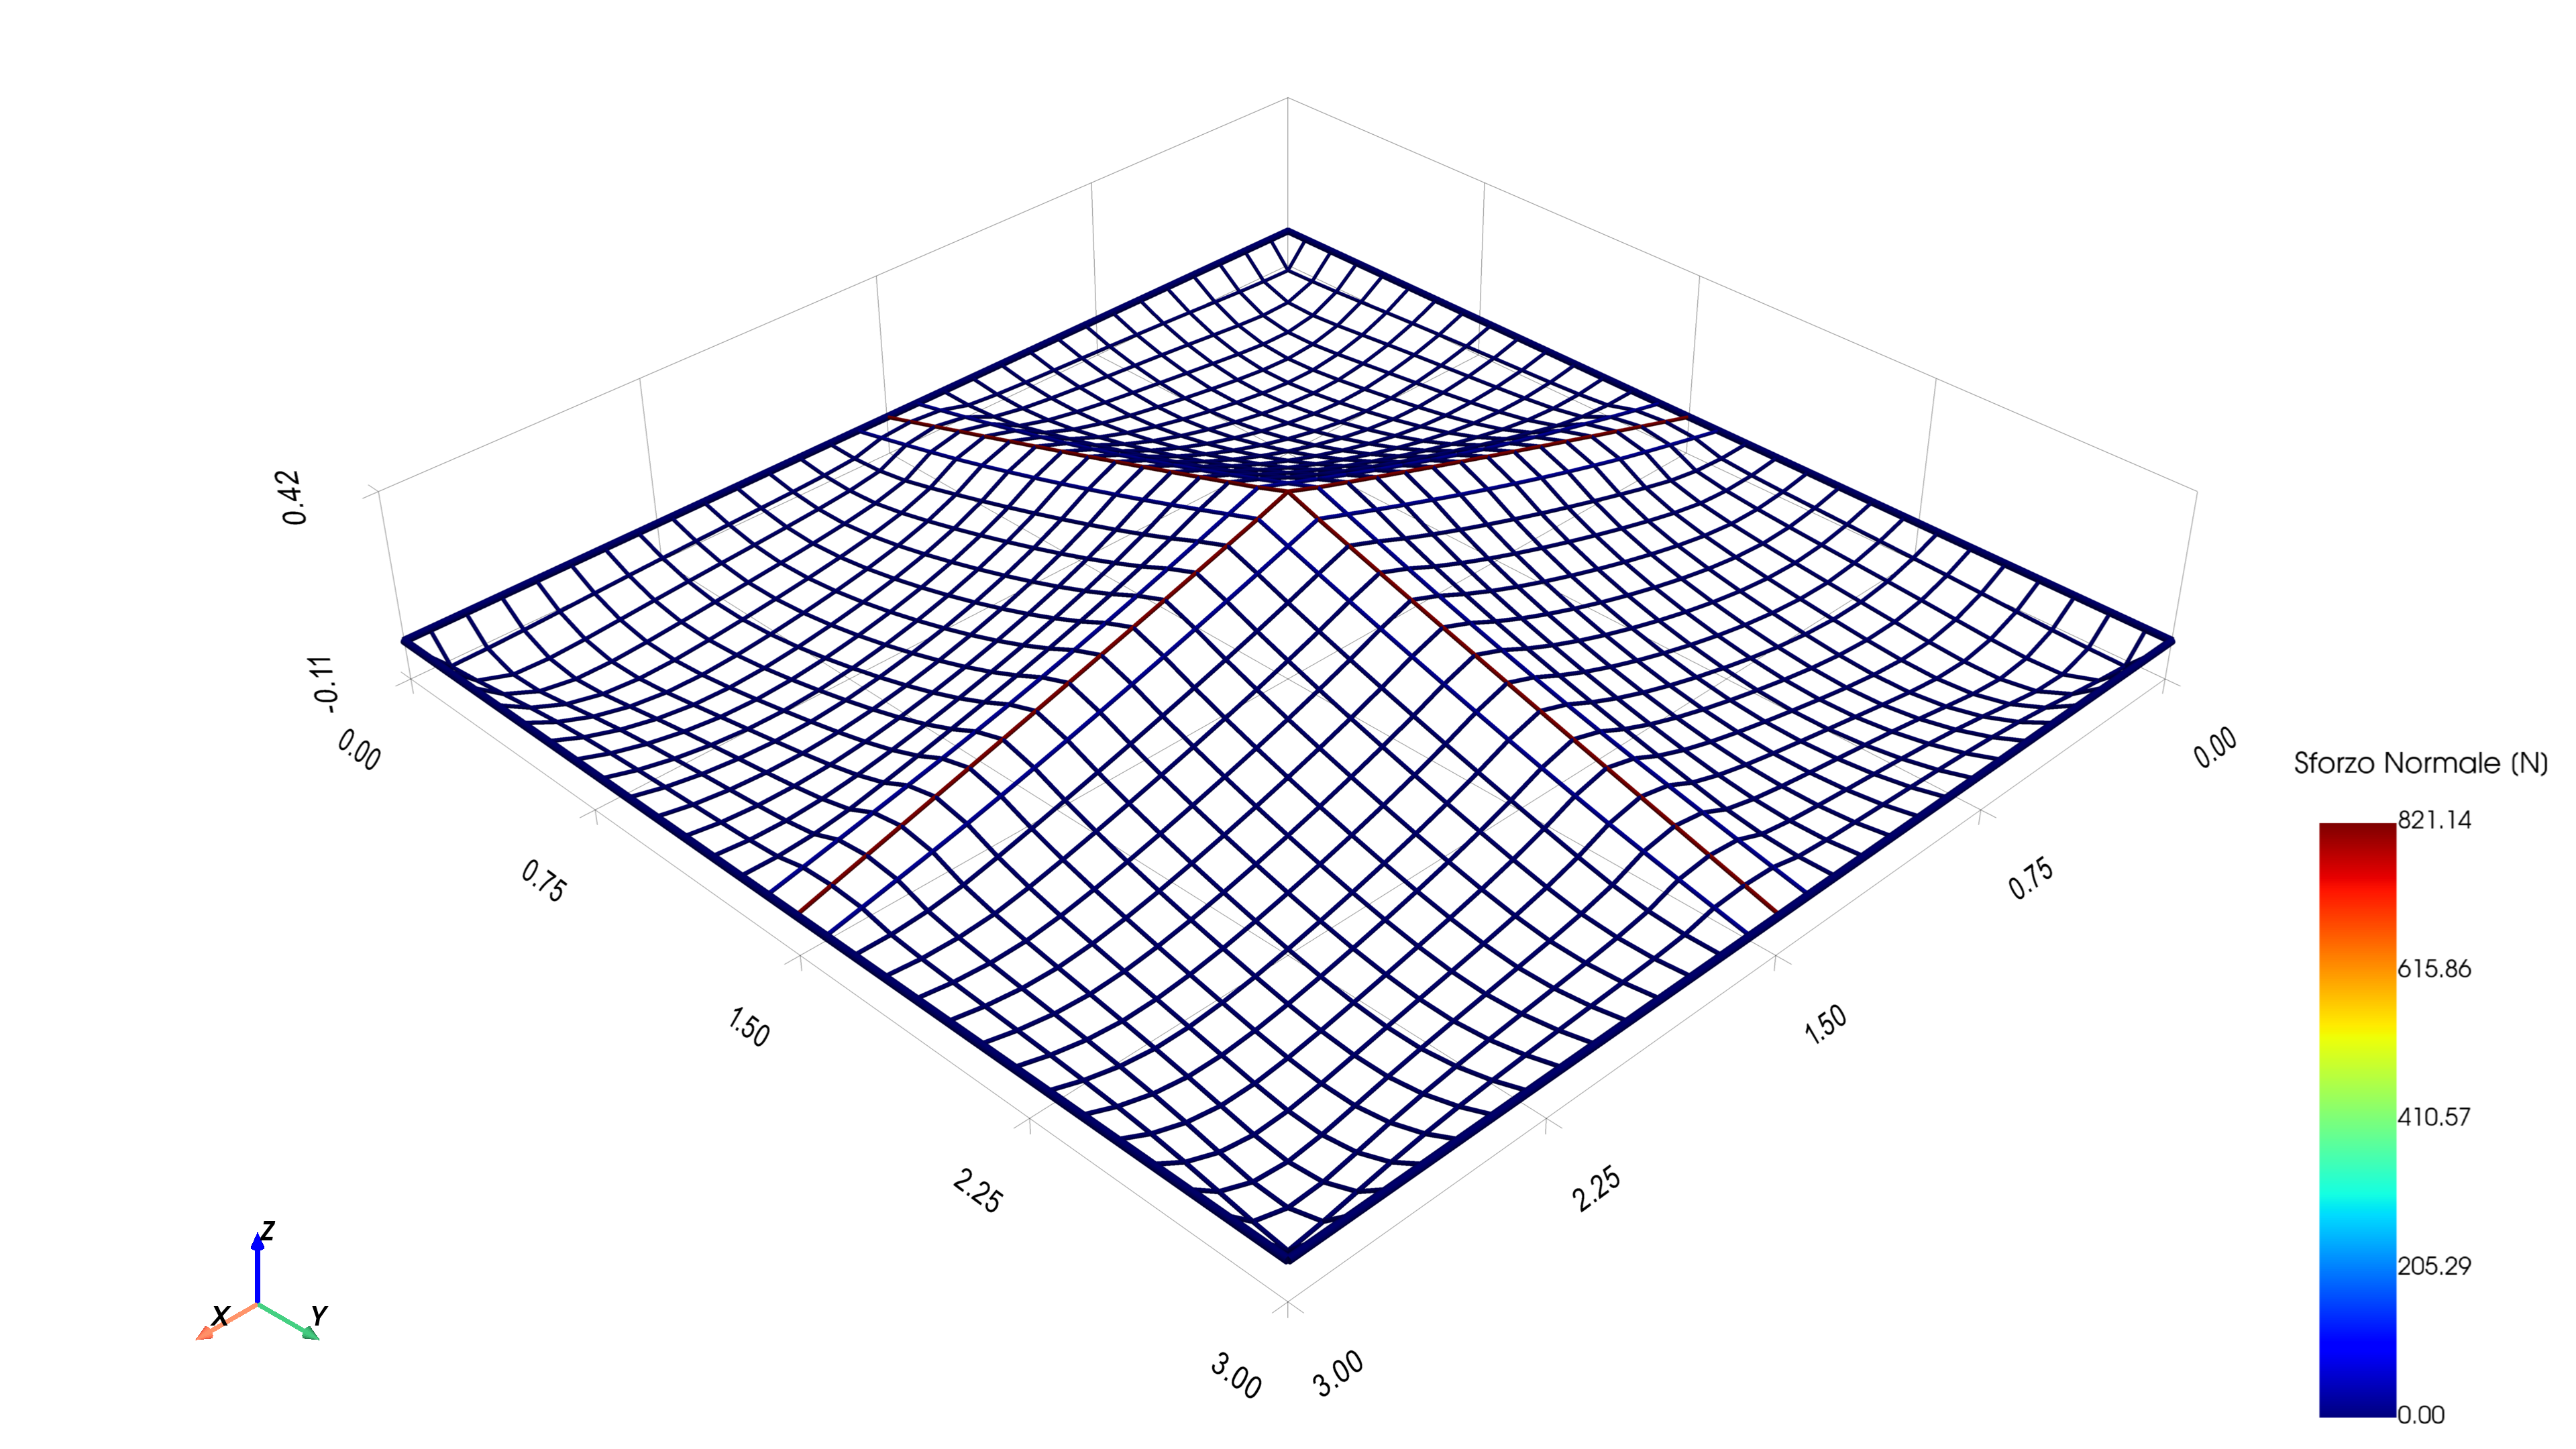
\includegraphics[width=\textwidth]{143_capitoli/capitolo4/immagini_capitolo_4/immagini_forza_concentrata/rete_forza_concentrata2.png}
    \caption{Rete soggetta all'azione del peso proprio e di una forza verticale applicata in mezzeria}
    \label{fig:forza_concentrata_verticale}
\end{figure}

\begin{figure}[H]
   \centering
    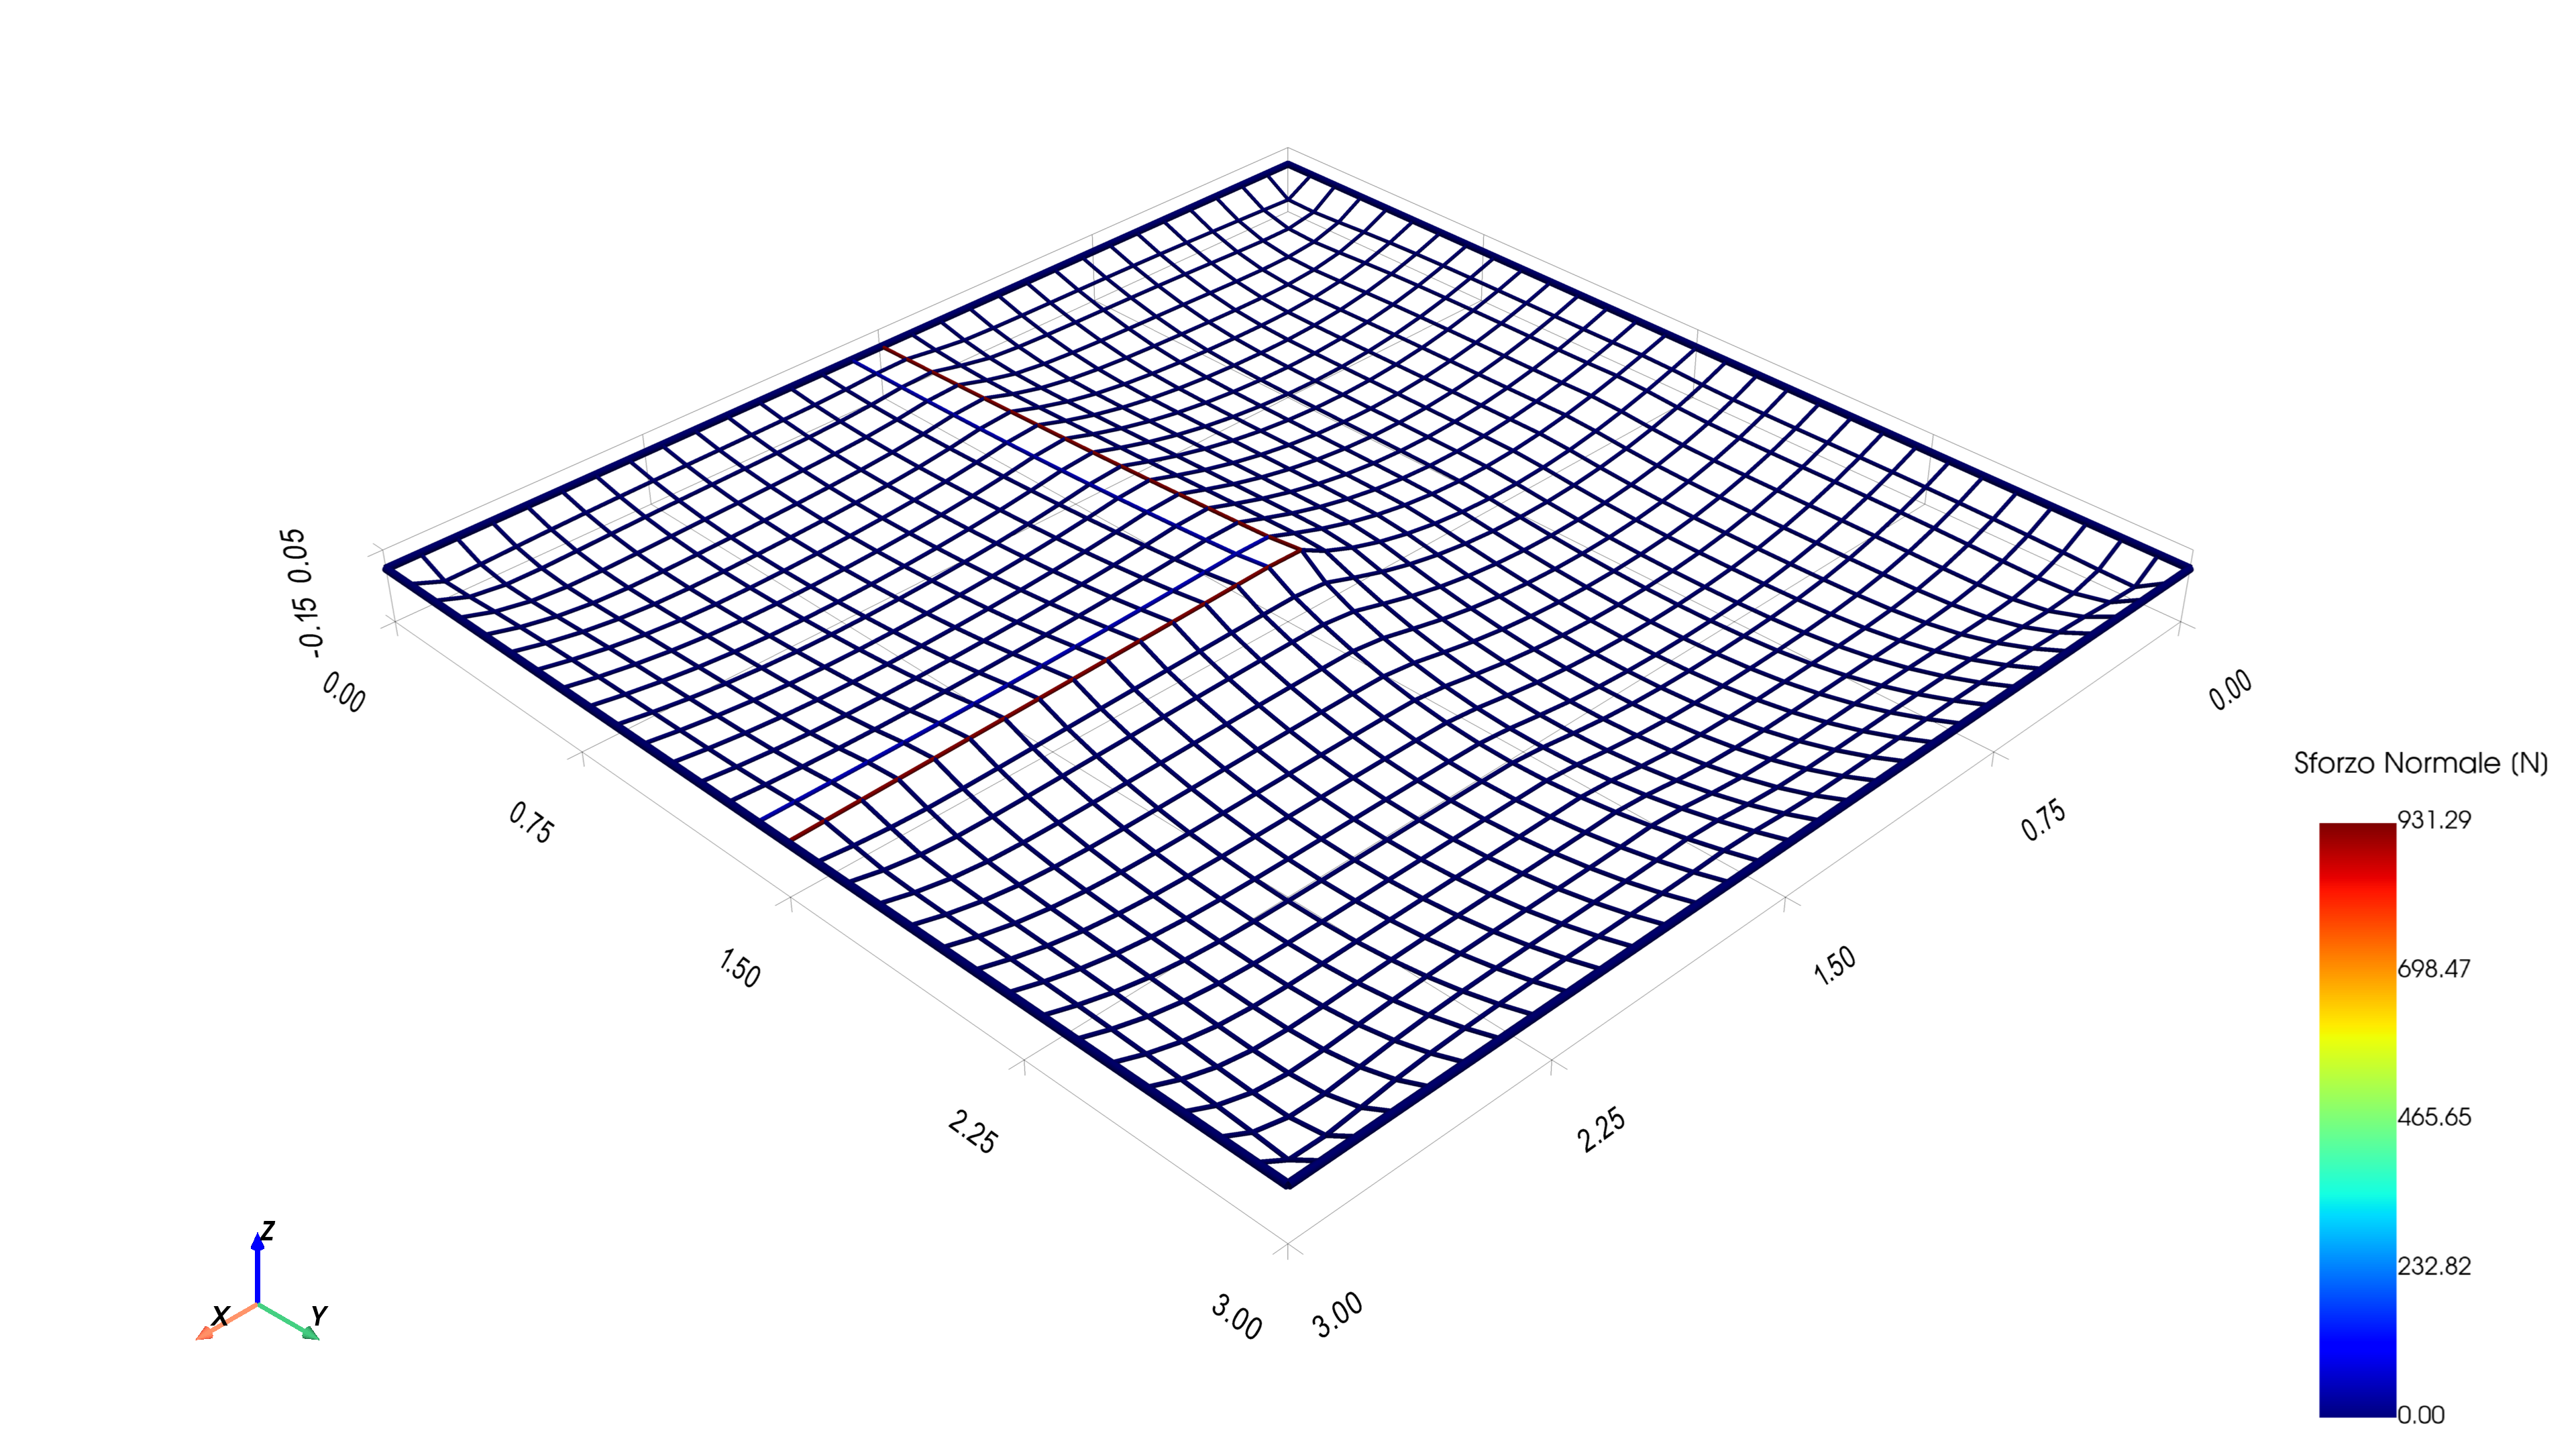
\includegraphics[width=\textwidth]{143_capitoli/capitolo4/immagini_capitolo_4/immagini_forza_concentrata/rete_forza_concentrata.png}
    \caption{Rete soggetta all'azione del peso proprio e di una forza inclinata applicata in mezzeria}
    \label{fig:forza_concentrata_inclinata}
\end{figure}

\begin{table}[htbp]
    \centering
    \caption{Proprietà geometriche e meccaniche delle reti soggette a carichi concentrati di \cref{fig:forza_concentrata_verticale,fig:forza_concentrata_inclinata}}
    \vspace{5pt}
    \label{tab:caratteristiche_reti_forze_concentrate}
    \begin{tabularx}{\textwidth}{l c X}
        \hline
        \textbf{Parametro} & \textbf{Simbolo} & \textbf{Valore nominale} \\ \hline
        Dimensione totale della rete & $L_x \times L_y$ & $3.00 \times 3.00$ $[\text{m}]$ \\
        Dimensione della singola maglia (Q) & $l_{m_x} \times l_{m_y}$ & $10 \times 10$ $[\text{cm}]$ \\
        Diametro nominale delle funi di maglia & $\phi _1$ & $5.0$ $[\text{mm}]$ \\       
        Diametro nominale delle funi di maglia & $\phi _2$ & $10.0$ $[\text{mm}]$ \\
        Modulo di elasticità longitudinale fune & $E$ & 2.1e9 $[\text{Pa}]$ \\
        Area della sezione trasversale fune & $A_1$ & 19.63 $[\text{mm}^2]$ \\
        Area sezione trasversale fune di bordo & $A_2$ & 78.54 $[\text{mm}^2]$ \\
        Regolarizzazione del legame costitutivo & $\beta$ & 1e6 $[-]$\\  
        Rapporto di laschezza \cref{fig:forza_concentrata_verticale} (entrambe le direzioni) & $\xi$ & 3.33 $[\%]$\\
        Rapporto di laschezza \cref{fig:forza_concentrata_inclinata} (entrambe le direzioni) & $\xi$ & 1 $[\%]$\\ \hline
    \end{tabularx}
\end{table}

\begin{table}[htbp]
    \centering
    \caption{Proprietà delle forze concentrate applicate nelle \cref{fig:forza_concentrata_verticale,fig:forza_concentrata_inclinata}}
    \vspace{5pt}
    \label{tab:caratteristiche_forze_concentrate}
    \begin{tabularx}{\textwidth}{l c X X}
        \hline
        \textbf{Parametro} & \textbf{Simbolo} & \textbf{Caso Verticale} \small{(\cref{fig:forza_concentrata_verticale})} & \textbf{Caso Inclinato} \small{(\cref{fig:forza_concentrata_inclinata})} \\ \hline
        Nodo di applicazione & - & Mezzeria  & Mezzeria  \\
        Componente $x$ & $F_x$ & $0.0$ $[\text{N}]$ & $-1000$ $[\text{N}]$ \\
        Componente $y$ & $F_y$ & $0.0$ $[\text{N}]$ & $1000$ $[\text{N}]$  \\
        Componente $z$ & $F_z$ & $1000$ $[\text{N}]$ & $100$ $[\text{N}]$ \\
        Modulo del vettore forza & $|\underline{F}|$ & $1000$ $[\text{N}]$ & $1417.14$ $[\text{N}]$ \\ \hline
    \end{tabularx}
\end{table}

\section{Reti soggette alla prova quasi statica}

Uno degli obiettivi del presente lavoro di tesi è valutare la capacità di assorbimento dell'energia elastoplastica di una rete di dimensioni reali, così da fornire al progettista uno strumento idoneo a stimare l'esito del superamento della prova di impatto dinamico di normativa come visto nel \cref{chap:capitolo3}. Per compiere tale analisi occorre caratterizzare meccanicamente gli elementi del modello numerico e validare i risultati ottenuti mediante il confronto con prove sperimentali di laboratorio. Poiché la normativa non richiede esplicitamente la valutazione dell'assorbimento energetico del dispositivo di intercettazione, i produttori non forniscono curve forza spostamento per la rete nel suo complesso.

Tuttavia, i produttori eseguono le prove quasi-statiche richieste dalle normative di settore per la caratterizzazione della rete impiegata nei vari sistemi tipologici. Tali dati sono forniti a corredo della documentazione tecnica del prodotto. Ai fini del presente lavoro di ricerca, si dispone dei risultati sperimentali relativi a una rete di geometria nota, gentilmente concessi dal retificio "La Rete Srl". Nel contesto della modellazione numerica, la prova quasi-statica costituisce la validazione e non l'input del solutore che è invece rappresentato dalle proprietà meccaniche del singolo elemento di cavo. 

Le caratteristiche meccaniche del singolo filo vengono dedotte a partire dai risultati della prova di trazione sulla maglia, eseguita secondo le prescrizioni della norma EN 1263-1 \cite{EN1263-1} (con metodologie di prova di cui alla EN 1806 \cite{ENISO1806-2002}) per determinare la resistenza a trazione e l'assorbimento energetico dell'elemento fino a rottura. Tali prove di trazione sulla singola maglia sono anch'esse disponibili sottoforma di grafico forza-spostamento grazie ai dati forniti dal produttore.

Il percorso di validazione prende avvio dalla definizione del legame costitutivo del singolo cavo sulla base dei dati di prova sulla maglia. Definito il comportamento $N$-$\Delta l_p$ dell'elemento, le relative proprietà vengono implementate nel solutore per riprodurre la prova quasi-statica di normativa su un provino di dimensioni $3\times3 \, \text{m}$. Il confronto positivo tra i risultati numerici e quelli sperimentali permetterà di validare il solutore e di estenere l'applicazione alla simulazione su scala reale dell'intera rete, permettendoci quindi di stimare con accuratezza ingegneristica la capacità globale di assorbimento dell'energia. 

\subsection{Caratterizzazione maccanica delle funi}
Al fine di caratterizzare il degrado delle caratteristiche meccaniche prodotto dall'invecchiamento naturale sulle reti poste in opera, la normativa EN 1263-1 \cite{EN1263-1} prevede che la capacità di assorbimento dell'energia della maglia di rete mediante test di trazione prodotto in accordo con la normativa EN ISO 1806 \cite{ENISO1806-2002}, sia determinata ad intervalli temporali prescritti e confrontata con lo stesso risultato ottenuto però allo stato come nuovo per la stessa rete. In tal modo è possibile così valutare il rispetto da parte del dispositivo delle previsioni in tema di degrado delle caratteristiche meccaniche poste inizialmente. Perciò i produttori dei sistemi di intercettazione dei dispositivi di protezione forniscono i valori di assorbimento dell'energia di una maglia di rete posta in trazione allo stato nuovo.

Il principio della prova definita dalla norma EN ISO 1806 prevede di estendere una maglia di rete fino a quando uno dei nodi o dei giunti (presenti agli angoli della maglia) raggiungono la forza di rottura. La prova è compiuta per mezzo di un apparato di test che registra la forza applicata e lo spostamento relativo compiuto dalle estremità a cui la maglia è attaccata. 

Non essendo completamente a conoscenza delle condizioni di prova con cui è stato ricavato il risultato grafico fornitoci dal produttore mediante il rapprto di prova i cui risultati sono riportati nella figura FARE RIFERIMENTO ALLA FIGURA, assumendo che le prove siano state eseguite in conformità con le prescizioni di norma, si assumerà, in accordo con le figure,  che la lunghezza iniziale del provino $\bar{l}_p$ sia pari a:
\begin{equation}
    \bar{l}_p = 2l_m - \frac{P_p}{2}
\end{equation}
considerato che la normativa EN ISO 1806 \cite{ENISO1806-2002} impone che il diametro del perno sia pari a $d_p = 2,0\,\text{cm}$, allora ne segue che per una maglia con lunghezza dei lati dichiarata di $l_m = 10 \, \text{cm}$, si avrà che $\bar{l}_p = 16,86 \, \text{cm}$.  

Dai dati in nostro possesso risulta quindi chiaro che non siano noti né il legame costitutivo di un elemento di rete impiegato nel modello, ma di un elemento di rete differente con lunghezza $l_p$ e area di sezione $A_p$ note, nè di un legame costitutivo, $\sigma - \epsilon$ come definito nel capitolo \cref{chap:capitolo2}, necessario per applicare la formulazione del PFEF presentata.

\subsection{Linearizzazione a tratti del legame}

\subsubsection{Approssimazione bilineare/trilineare/quadrilineare}

\subsubsection{Caratterizzazione meccanica dell'elemento di fune}
La legge costitutiva forza-allungamento $N(\Delta lp)$ è ricavata sperimentalmente su un provino di lunghezza $l_p$ e area resistente $a_p$. Per ottenere la corrispondente legge dell'elemento generico della rete, di lunghezza iniziale $l_e$ e area $a_e$, si applica una scalatura diretta basata sull'allungamento. 

Poichè lo \textit{stretch} $\lambda$ di un elemento sottoposto a solo sforzo normale monoassiale è adimensionale e definito come:
\begin{equation}
    \lambda =  \frac{l}{\bar{l}}
\end{equation}
Allora tale misura della variazione di lunghezza tra le due configurazioni è invariante rispetto all'elemento a cui è applicata, per cui: 
\begin{equation}
    \lambda = \lambda_p = \lambda_e
\end{equation}
Essendo la componente del tensore delle deformazioni di Green-Lagrange in direzione assiale dell'asta, esprimibile in funzione dello \textit{stretch}:
\begin{equation}
    e_{11} = \frac{1}{2} \frac{l_e^2 - \bar{l}_e^2}{\bar{l}_e^2} = \frac{1}{2} (\lambda^2 - 1)
\end{equation}
possiamo concludere che:
\begin{equation}
     e_{11} = e_{11,e} = e_{11,p} 
\end{equation}
Rircordando l'espressione della deformazione di Green-Lagrange ed imponendo l'uguaglianza si ottiene che: 
\begin{equation}
    \frac{\Delta l_p}{l_p} = \frac{\Delta l_e}{l_e}
\end{equation}
Perciò risulta che: 
\begin{equation}
    \Delta l_e = \Delta l_p \frac{l_e}{l_p} 
\end{equation}
La forza assiale invece può essere scalata, in virtù della definizione dello sforzo normale, considerando che la componente del secondo tensore di Piola-Kirchhoff è dipendente solamente dalla misura di deformazione di Green-Lagrange, secondo la relazione: 
\begin{equation}
    N = \bar{a} \, s_{11}(e_{11})\lambda
    \label{eq:N_s_11}
\end{equation}
Dall'equivalenza della componente del secondo tensore di Piola-Kirchhoff, a fronte dello stesso valore della componente di deformazione del tensore di Green-Lagrange, otteniamo la seguente relazione:
\begin{equation}
    N_e = N_p \, \frac{\bar{a}_e}{\bar{a}_p} 
\end{equation}
Di conseguenza, il valore di rigidezza tangente dell'elemento può essere espressa in funzione del valore di rigidezza tangente del provino, secondo la relazione:
\begin{equation}
    k_{e} = k_{p} \, \frac{\bar{a}_e \bar{l}_p}{\bar{a}_p \bar{l}_e}  
\end{equation}

La legge costitutiva sperimentale dell'elemento è adesso espressa come relazione forza-allungamento $N(\Delta l_e)$, dove $\Delta l_e = l_e -\bar{l}_e$ rappresenta la differenza di lunghezza dell'elemento in configurazione di riferimento, rispetto alla configurazione corrente. Nella formulazione del PFEF che adotteremo, tuttavia, lo sforzo normale è espresso rispetto allo \textit{stretch}. Il passaggio da $\Delta l_e$ a $\lambda$ è immediato, poiché:
\begin{equation}
    \Delta l_e = \bar{l}_e\left(\lambda - 1 \right)
\end{equation}
Pertanto, la legge costitutiva può essere riscritta come: 
\begin{equation}
    N_e\left(\Delta l_e\right) = N(\bar{l}_e\left(\lambda - 1 \right))
\end{equation}
La riscrittura della legge in funzione di $\lambda$ consente inoltre di ottenere in modo diretto la rigidezza tangente rispetto allo \textit{stretch}:
\begin{equation}
    k_{\lambda} = \frac{dN}{d\lambda} = \frac{dN}{d(\Delta l)} \frac{d(\Delta l)}{d\lambda} = k \, \bar{l}
\end{equation}
Che per l'elemento $e$-esimo della rete di funi assume la forma: 
\begin{equation}
    k_{e,\lambda} = k_e \, \bar{l}_e
    \label{eq:k_lambda}
\end{equation}  

\subsection{Formulazione alternativa dell'elemento cavo PFEF}
La formulazione del PFEF vista precedentemente nel \cref{chap:capitolo2} esprimeva le matrici di rigidezza secante e tangente dell'elemento $e$-esimo del sistema sotto le ipotesi di un legame costitutivo $\sigma$-$\epsilon$ elastico lineare sotto l'ipotesi di piccoli spostamenti. Data la necessità di esprimere il PFEF in funzione del legame costitutivo dell'elemento cavo rispetto allo \textit{stretch} e di eliminare l'ipotesi di piccole deformazioni, è quindi necessario procedere ad una nuova formulazione dell'elemento cavo da impiegare all'interno della formulazione del PFEF descritta in Valvo \cite{Valvo1,Valvo2}. 

In Valvo \cite{Valvo1,Valvo2}, assumendo funzioni di forma lineari per gli elementi, la matrice di rigidezza elastica secante $S_e \in \mathbb{R}^{6\times6}$ e la matrice di rigidezza elastica tangente $T_e \in \mathbb{R}^{6\times6}$ sono espresse come segue: 
\begin{equation}
   S_e(\underline{x}_e) = s_{11} \, \frac{\bar{a}_e}{\bar{l}_e} \left[ \Delta \right]
   \label{eq:matrice_secante_gd}
\end{equation}
\begin{equation}
   T_e\left(\underline{x}_e\right) = S_e\left(\underline{x}_e\right) + C_{1111} \frac{\overline{a}_e}{\overline{l}_e^3} \left[ \Delta \right]\,\underline{x}_e {\underline{x}_e}^T \left[ \Delta \right] 
   \label{eq:matrice_tangente_gd}
\end{equation}
dove $C_{1111}$ è definito come: 
\begin{equation}
    C_{1111} = \frac{\partial^2 \bar{\varphi}}{{\partial e_{11}}^2}
\end{equation}
Ricordando che l'espressione della componente del secondo tensore di Piola-Kirchhoff può essere espressa come: 
\begin{equation}
    s_{11} = \frac{\partial \bar{\varphi}}{\partial e_{11}}
\end{equation}
Allora: 
\begin{equation}
    C_{1111} = \frac{\partial s_{11}}{\partial e_{11}}
\end{equation}
che per la regola della catena può essere scritto:
\begin{equation}
    C_{1111} = \frac{\partial s_{11}}{\partial \lambda}\frac{\partial \lambda}{\partial e_{11}}
    \label{eq:C1111}
\end{equation}

Esprimendo $s_{11}$ secondo l'equazione \eqref{eq:N_s_11} e compiendo le derivate si arriva all'espressione:
 \begin{equation}
    C_{1111} = \frac{1}{\lambda} \frac{\partial s_{11}}{\partial \lambda} = \frac{1}{\bar{a}_e{\lambda}^3} \left( \frac{\partial N(\lambda)}{\partial \lambda} \lambda - N(\lambda)\right)
    \label{eq:C1111_2}
\end{equation}
Sostituendo nell'espressione \eqref{eq:matrice_tangente_gd}, le espressioni delle matrici di rigidezza elastica secante e tangente assumono la forma: 
\begin{equation}
   S_e(\underline{x}_e) = \frac{N(\lambda)}{l_e} \left[ \Delta \right]
   \label{eq:matrice_secante_gd2}
\end{equation}
\begin{equation}
   T_e\left(\underline{x}_e\right) = S_e\left(\underline{x}_e\right) +  \frac{K(\lambda)\lambda - N(\lambda)}{l_e^3}\,[\Delta]\underline{x}_e\underline{x}_e^T[\Delta]
   \label{eq:matrice_tangente_gd_2}
\end{equation}

Assumendo un legame costitutivo lineare a tratti in funzione del valore $\lambda_1$ può essere espresso come: 
\begin{equation}
   N(\lambda_1) = 
\begin{cases}
    0 \,  & \text{se } \lambda_1 \leq 0 \\[6pt]
    K_1    \, \lambda_1, & \text{se } \lambda_{y1} \geq \lambda_1 \geq 0 \\[6pt]
    \dots\\[6pt]
    N(\lambda_{yT-1}) + K_T    \, (\lambda_1 - \lambda_{yT-1}), & \text{se } \lambda_{yT} \geq \lambda_1 \geq \lambda_{yT-1} \\[6pt]
    N(\lambda_{yT}) + K_{T+1}  \, (\lambda_1 - \lambda_{yT})  & \text{negli altri casi } 
\end{cases}
\label{eq:tension_only2_gd}
\end{equation}
Allora la derivata parziale dello sforzo normale $N(\lambda_1)$ rispetto a $\lambda_1$ diventa: 
\begin{equation}
    K(\lambda_1) = 
\begin{cases}
    0 \,    & \text{se } \lambda_1 \leq 0 \\[6pt]
    K_1     & \text{se } \lambda_{y1} \geq \lambda_1 \geq 0 \\[6pt]
    \dots\\[6pt]
    K_T     & \text{se } \lambda_{yT} \geq \lambda_1 \geq \lambda_{yT-1} \\[6pt]
    K_{T+1} & \text{negli altri casi } 
\end{cases}
\label{eq:tension_only2_gd_k}
\end{equation}
e l'espressione \eqref{eq:matrice_tangente_gd_2} assume la forma: 
\begin{equation}
   T_e\left(\underline{x}_e\right) = S_e\left(\underline{x}_e\right) + \frac{\left( K_T - N(\lambda)\right)}{l_e^3} \left[ \Delta \right]\underline{x}_e\underline{x}_e^T[\Delta]
   \label{eq:matrice_tangente_gd_4}
\end{equation}
Ponendo che:
\begin{equation}
    \underline{n}_e = \frac{1}{l_e} \left[ \Delta \right] \underline{x}_e 
    \label{eq:prodotto_esterno}
\end{equation}
Introducendo le espressioni \eqref{eq:k_lambda} \eqref{eq:matrice_secante_gd} e \eqref{eq:prodotto_esterno}, otteniamo che:
\begin{equation}
   T_e\left(\underline{x}_e\right) = \frac{N(\lambda)}{l_e} \left[ \Delta \right] + \frac{\left( k_e l_e - N(\lambda)\right)}{l_e} \underline{n}_e \underline{n}_e^T
   \label{eq:matrice_tangente_gd_5}
\end{equation}



\subsubsection{Condizioni di vincolo}
\subsubsection{Configurazione iniziale}





